\chapter{低轨卫星网络链路洪泛攻击的多签名在网检测与队列缓解}
\label{chap:ms_satshield}

\section{引言}
大规模低轨卫星网络通过星间链路与星地链路为全球提供低时延、广覆盖的互联网接入。然而，与地面骨干网类似，LSN 作为高价值通信基础设施同样面临拒绝服务类攻击风险，其中以链路洪泛攻击尤为突出。LFA 的典型策略是利用分布式受控终端（bots）发起大量看似正常的低速流量，将其沿着特定路径汇聚到目标链路，从而在链路上形成拥塞，甚至阻断重要区域间通信。ICARUS 工作系统化刻画了面向 LSN 的 LFA 攻击面与攻击构造过程，指出攻击者可以借助公开轨道信息推测路由，并在拓扑动态变化下持续调整攻击流集合以维持链路拥塞，从而对 LSN 的可用性形成实质威胁\citess{icarus}。

从防御角度看，LSN 的网络形态使传统的控制面集中检测、再下发策略的闭环方案难以满足实时性。一方面，卫星网络控制通道的带宽和时延都较为受限，跨星或星地的控制闭环通常达到毫秒到十毫秒量级；另一方面，攻击流集合可能在亚秒级甚至更短时间尺度内变化，控制面统计汇聚与策略更新一旦滞后，防御效果就会明显下降。SatShield 针对这一问题提出将检测与缓解尽量下沉到数据平面：以地址聚合速率作为区分特征，在数据平面持续维护近似 top-$K$ 重流候选，并通过队列调度实现被动丢弃，从而达到近实时的在网缓解\citess{satshield}。


% [INS-2026-CH3-01]
这一问题在 2025--2026 年更加突出。随着 Starlink Direct to Cell 开始直接承载面向普通 LTE 终端的接入业务，Amazon Leo 推出面向企业与政府场景的私网互连和千兆级终端，以及 IRIS$^2$ 等体系把关键基础设施连接纳入星座目标函数，LEO 网络上合法的大流、回传流和云互连流都在增多\citess{starlink_direct_to_cell_2026, amazon_leo_enterprise_2025, eu_iris2_2024}。继续把重流直接视为可疑对象，误判风险会更高，因此检测逻辑需要把速率与扇入、扇出、跨窗口持续性等结构特征合并考虑。本章提出 MS-SatShield，就是针对这种业务多样化背景下的可分性下降。

尽管 SatShield 已证明聚合速率在现有卫星系统约束下具有较好的可分性，但只依赖速率特征仍会遇到两类难以回避的问题。真实网络中的正常业务本身就存在长尾与大流现象，例如热门服务和突发上行，仅用速率很难区分合法大流与攻击聚合。与此同时，攻击者还可以通过扩大 bot 规模、降低单 bot 速率，或将攻击流量分摊到更多 decoy 目的，削弱单一聚合维度上的速率差异，使一级候选生成质量下降，进而诱发漏检或误检。SatShield 在讨论部分也指出，随着 bot 规模和业务形态继续演进，引入 fan-in/fan-out 等结构性签名是提高鲁棒性的自然方向\citess{satshield}。地面网络中，Ripple\citess{ripple} 和 Mew\citess{mew} 已展示了基于可编程数据面的 LFA 防御潜力，但它们依赖于地面交换芯片更充裕的存储与计算资源，无法直接移植到 SWaP 受限的星载环境。

基于上述背景，本章在 SatShield 的一级候选生成与队列调度缓解框架上，提出一种多签名在网检测与缓解方法（MS-SatShield）。该方法以 CMS 频率估计与固定容量候选缓存构成一级候选生成器，避免全量 distinct 统计带来的状态爆炸；同时在候选集合上引入 fan-in/fan-out 与持续性（persist）等结构性特征，以提升对多 decoy 分摊、脉冲式 on-off 和速率下沉等退化策略的检测鲁棒性，并将多签名可疑度映射为队列优先级，实现快速、低误伤的攻击缓解。

\section{问题定义与方法设计}
\subsection{威胁模型与问题表述}
将 LSN 在时刻 $t$ 表示为动态图 $G(t)=(V,E(t))$，其中 $V$ 为卫星节点集合，$E(t)$ 为随时间变化的星间链路集合。每条链路 $e\in E(t)$ 具有容量 $C_e$。在 LFA 场景中，攻击者控制一组分布式终端（bots）集合 $\mathcal{B}$，并选择一组 decoy 目的集合 $\mathcal{D}$，使得从 $\mathcal{B}$ 到 $\mathcal{D}$ 的攻击流量在转发路径上穿越目标链路 $e^\star$，从而使 $e^\star$ 的负载超过其容量并发生拥塞。与地面网络中常见的五元组拆分类似\citess{crossfire}，攻击者可通过多对多配对（一个 bot 对多个目的、一个目的由多个 bot 访问）将单条五元组流的速率降低到接近正常水平，但这会显著改变流量的结构性特征，例如源的 fan-out、目的的 fan-in 以及可疑 key 的持续出现模式\citess{satshield}。

% [INS-ICARUS-08]
为与 ICARUS 的攻击评估语义保持一致，本章将攻击有效性分为两类目标：一类关注目标链路是否达到拥塞阈值，另一类关注达成这一目标需要付出多大的可见代价。前者由目标链路是否超容表征，后者分别由攻击成本（达到拥塞所需注入总带宽）与可检测性代理指标（上行侧最大增量 maxUp）刻画。本文聚焦检测与缓解机制本身，不直接求解最优攻击流分配，但在指标解释上沿用这一语义，以便与 ICARUS/SatShield 的结果保持可对齐性\citess{icarus}。

为了与可编程交换机的周期性统计与配置机制对齐，本章采用固定时间窗口 epoch建模。记第 $t$ 个 epoch 的时间长度为 $\Delta$，在该窗口内对某类地址 key（源地址或目的地址）进行聚合统计。对任意 key $a$，定义其在 epoch $t$ 内的聚合字节数与聚合速率分别为
\begin{equation}
\text{bytes}_t(a)=\sum_{p\in \mathcal{P}_t(a)} len(p),\qquad
R_t(a)=\frac{\text{bytes}_t(a)}{\Delta},
\label{eq:rate_def}
\end{equation}
其中 $\mathcal{P}_t(a)$ 表示 epoch $t$ 内地址字段取值为 $a$ 的数据包集合，$len(p)$ 为包长。

为刻画结构性特征，记每个包还包含一个与 key 互补的对端字段 $x$：当以源地址作为 key 时，$x$ 为目的地址；当以目的地址作为 key 时，$x$ 为源地址。则可定义 key 的 distinct 对端规模：
\begin{equation}
F_t(a)=\left|\{x \mid (a,x)\ \text{在 epoch}\ t\ \text{内出现}\}\right|,
\label{eq:fan_def}
\end{equation}
其中 $F_t(a)$ 在源 key 模式下对应 fan-out（FO），在目的 key 模式下对应 fan-in（FI）。

此外，考虑 LSN 拓扑与流量均具有动态性，单一窗口内的一级候选结果可能出现抖动。为提升稳定性，引入持续性特征（persist），表示某 key 在最近 $k_p$ 个 epoch 中进入候选集合的次数：
\begin{equation}
P_t(a)=\sum_{i=1}^{k_p}\mathbf{1}\left[a\in \mathcal{H}_{t-i}\right],
\label{eq:persist_def}
\end{equation}
其中 $\mathcal{H}_{t}$ 表示基于 epoch $t$ 窗口统计结果导出的一级候选 key 集合，$\mathbf{1}[\cdot]$ 为指示函数。

需要指出的是，速率退化与结构性特征放大之间并非彼此独立。考虑 $|\mathcal{B}|$ 个 bot 向 $M$ 个 decoy 目的发起攻击，记每个 bot 平均访问 $d$ 个 decoy（$1\le d\le M$），并假设 bot 的发送速率在其访问的 decoy 上近似均分。令总攻击注入量为 $A=\sum_{b\in\mathcal{B}}r_b$，则单个 decoy 的聚合速率仍约为 $R_{\text{atk}}\approx A/M$，而结构特征满足
\begin{equation}
\mathrm{FO}_{\text{bot}} = d,\qquad
\mathbb{E}[\mathrm{FI}_{\text{decoy}}] = \frac{|\mathcal{B}|\,d}{M}.
\label{eq:fi_lower}
\end{equation}
特别地，当每个 bot 仅访问一个 decoy（$d=1$）时，有 $\mathrm{FO}_{\text{bot}}=1$，且 $\mathbb{E}[\mathrm{FI}_{\text{decoy}}]=|\mathcal{B}|/M$。因此，在固定总攻击预算 $A$ 的条件下，攻击者虽然可以通过增大 $M$ 压低按目的地址聚合后的速率，但往往会在 fan-in 或 fan-out 的至少一维上保留结构性痕迹。更准确地说，攻击者并非在任何条件下都无法同时压低速率与结构特征；但在本文考虑的攻击预算、bot 规模与终端速率约束下，压低 per-key 聚合速率通常会推动 FI/FO 中至少一维偏离良性区间，因此多签名检测相较于单一速率检测具有更强的鲁棒性。

在本章后续实验中，除非另行说明，均以目的地址作为 key，从而 $F_t(a)$ 对应 fan-in（FI），衡量访问同一目的地的不同源地址数量。

本章关注的问题是：在星载可编程交换机片上存储和流水线算力都受限的条件下，如何在每包线速处理的前提下，利用 \emph{sketch 频率估计 + 显式候选缓存} 在线恢复当前窗口内的重 key 候选集合，并在该候选集合上提取 $R_t(a)$、$F_t(a)$、$P_t(a)$ 等多维特征，进一步为可疑 key 分配不同的队列优先级，实现对 LFA 的快速缓解，同时尽量降低对良性业务的误伤。

\subsection{预实验：速率可分性退化与多签名动机}
在给出正式系统设计之前，本文先用一个预实验说明单一速率特征在退化攻击下如何失效，并据此引出后续的多签名设计。SatShield 的一个重要观察是，在现有 LEO 系统约束下，攻击者若要使目标 ISL 达到拥塞，必须注入接近链路容量量级的总攻击流量；但受单终端上行能力、单星可服务用户数等约束，攻击流按源地址或目的地址聚合后，仍会呈现 Mb/s 量级的重尾分布，因此与绝大多数良性聚合速率之间存在可分性\citess{satshield}。基于这一观察，本章采用与 SatShield 一致的 LEO 仿真与流量构造思路：使用 Starlink Shell 1 星座拓扑（1584 颗卫星）和 ISL 容量 $20$~Gb/s 作为基本网络模型，良性背景流量由 CAIDA 匿名互联网 trace（CAIDA Anonymized Internet Traces 2018 数据集，采集自 Equinix-Chicago 监测点）经重放得到，并通过人口分布模型映射到城市对之间的通信需求（映射方法详见文献\citess{satshield} 第~IV-A~节）。该 trace 采集于 2018 年，与当前互联网流量分布可能存在差异，但本文关注的是攻击侧与正常侧的相对可分性，良性分布的绝对形状对结论影响有限。

图~\ref{fig:ch3_fig1_cdf} 以 $2\times2$ 子图展示了不同 decoy 数 $M$ 下，良性与攻击流量在每个地址 key 聚合速率维度上的经验分布函数（CDF）。绘制过程如下：先在仿真中固定 epoch 长度 $\Delta$，对每个 epoch 统计所有 key 的 $\text{bytes}_t(a)$，由式~(\ref{eq:rate_def}) 得到 $R_t(a)$；再分别对良性与攻击 key 集合绘制 CDF 曲线。当 $M=1$ 时，良性 $p_{99}\approx485$~Mb/s 与攻击聚合速率 $10{,}024$~Mb/s 之间存在约 $21$ 倍间隙；$M=10$ 时这一间隙缩小到约 $2$ 倍；$M=100$ 时攻击 key 速率下降到 $100$~Mb/s，已经落入良性分布的长尾区间；$M=1000$ 时攻击 key 与良性 key 基本重叠。该图展示了可分性随 $M$ 增大而退化的过程，也为后续多签名检测（图~\ref{fig:ch3_fig2_f1}）提供了动机。

\begin{figure}[!htb]
  \centering
  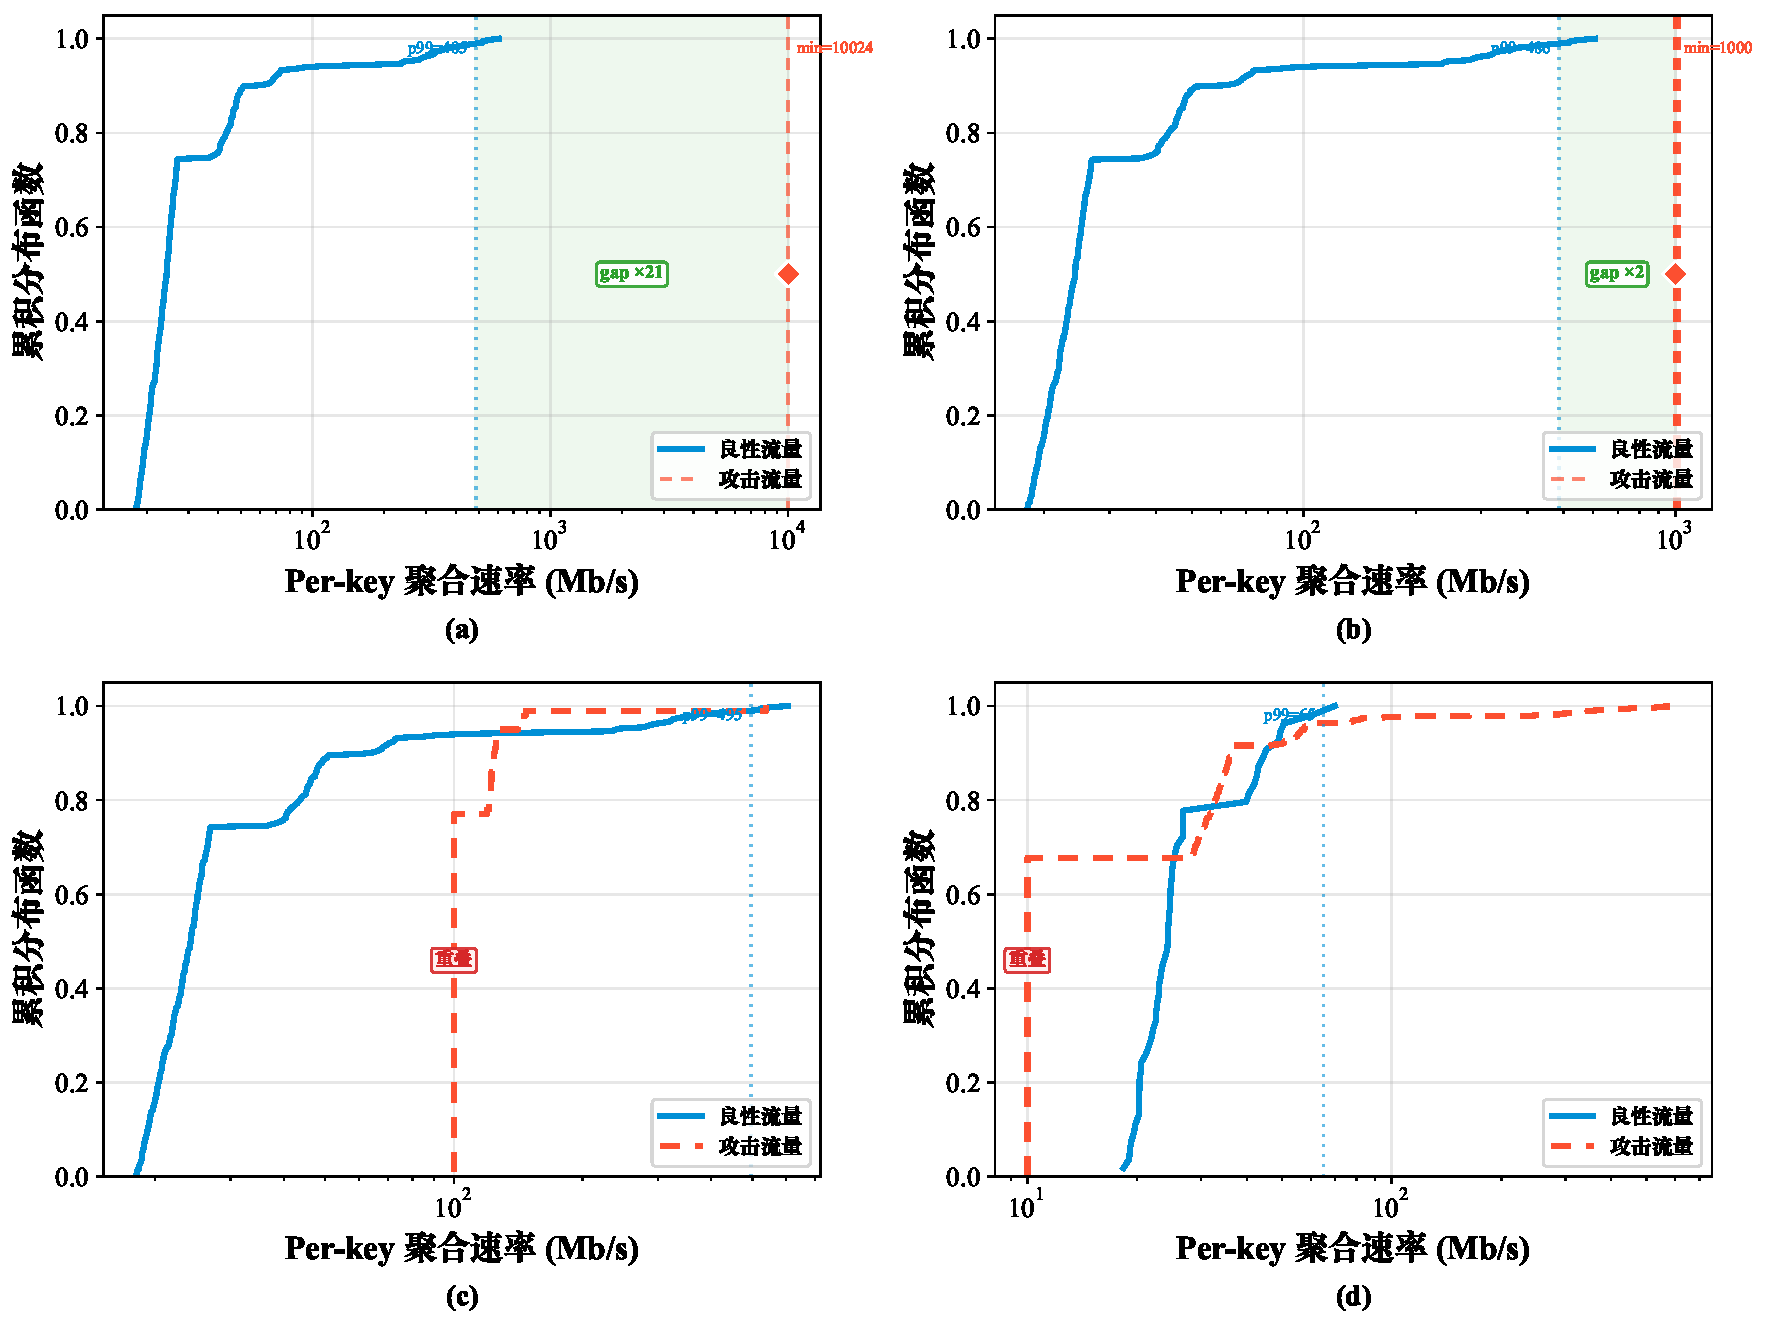
\includegraphics[width=0.92\linewidth]{figs/ch3/fig3_1_cdf.pdf}
  \caption{可分性随 decoy 数 $M$ 退化的 CDF 对比。四个子图分别对应 $M=1,10,100,1000$，蓝色实线为良性 key 聚合速率 CDF，红色虚线为攻击 key 聚合速率 CDF（$M\leq10$ 时因攻击 key 数量少，改用垂直线与散点标注）。绿色阴影区标注可分性间隙及倍数，红色 overlap 标注表示攻击与良性分布已交叉。}
  \label{fig:ch3_fig1_cdf}
\end{figure}

需要说明的是，图~\ref{fig:ch3_fig1_cdf} 中的可分性并非在任何条件下都成立。当攻击者采用更强的隐蔽策略时，速率特征可能退化并与良性长尾区间发生重叠。为明确方法的适用边界，并给出后续实验的退化路径，本章构造了三类典型设定：增大 bot 规模并降低单 bot 速率、将攻击流量分摊到更多 decoy 目的，以及采用脉冲式 on-off 策略使攻击 key 在窗口边界附近间歇出现。它们都满足 LFA 的基本约束，即总攻击注入量需要与目标链路剩余容量处于同一量级\citess{crossfire}：
\begin{equation}
\sum_{b\in\mathcal{B}} r_b \approx C_{e^\star}-U^{\text{benign}}_{e^\star},
\label{eq:lfa_budget}
\end{equation}
其中 $r_b$ 为 bot $b$ 的攻击发送速率，$U^{\text{benign}}_{e^\star}$ 为目标链路上良性占用带宽。式~(\ref{eq:lfa_budget}) 说明：如果希望将每个 key 的聚合速率压低到良性长尾附近，通常需要相应扩大可用 bot 数量或增大 decoy 分摊规模。如式~(\ref{eq:fi_lower}) 所示，这一过程中 fan-in/fan-out 至少一维往往会被放大，从而为多签名检测保留可利用的结构性痕迹。

\subsection{系统总览与数据流解释}
图~\ref{fig:ch3_fig5_arch} 展示了 MS-SatShield 的总体架构。系统由数据平面与星上代理（轻量控制平面）协同完成闭环：数据平面负责以线速维护基于 CMS 与候选缓存的一级候选生成摘要，并对活动候选执行轻量特征更新；星上代理以 epoch 为粒度拉取候选统计并计算多签名可疑度，将结果映射为队列优先级配置，再写回交换机用于下一轮调度。

\begin{figure}[!htb]
  \centering
  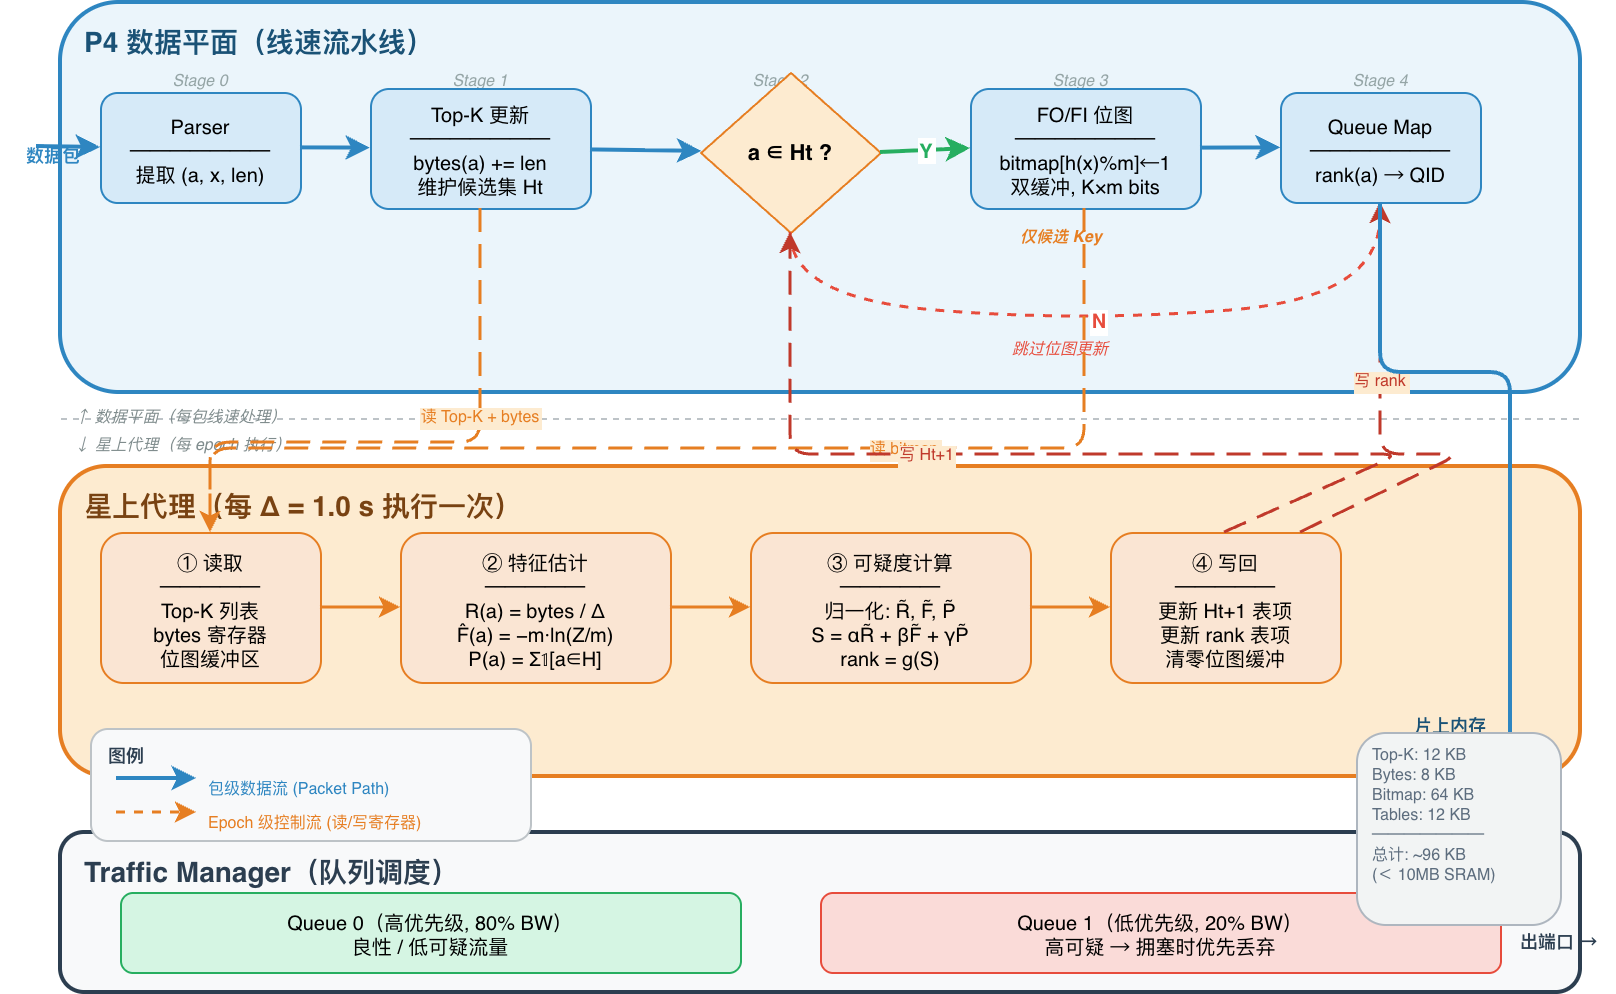
\includegraphics[width=0.96\linewidth]{figs/ch3/fig3-5_architecture.png}
  \caption{MS-SatShield 总体架构。数据平面逐包完成报文解析、CMS 与候选缓存更新、活动候选判定、FO/FI 位图更新与队列映射；星上 Agent 在每个 epoch 末读取候选摘要、字节统计与活动候选位图，估计速率、结构特征与持续性，生成下一轮活动候选配置与队列优先级映射，并写回交换机后由流量管理模块执行高/低优先级两队列调度。}
  \label{fig:ch3_fig5_arch}
\end{figure}

为了便于从处理流程理解图~\ref{fig:ch3_fig5_arch}，下面分别说明包级数据流与 epoch 级控制流。为避免时序歧义，本文保留 $\mathcal{H}_t$ 与 $\text{rank}_t(\cdot)$ 表示基于 epoch $t$ 统计结果导出的观测候选集与观测优先级，并记
\[
\mathcal{H}_t^{\mathrm{act}}=\mathcal{H}_{t-1},\qquad
\text{rank}_t^{\mathrm{act}}=\text{rank}_{t-1}.
\]
因此，在 epoch $t$ 的包处理中，交换机实际使用的是上一窗口导出的活动配置 $(\mathcal{H}_t^{\mathrm{act}},\text{rank}_t^{\mathrm{act}})$；而 epoch $t$ 结束后，代理根据当前窗口统计结果计算新的 $(\mathcal{H}_t,\text{rank}_t)$，并将其写回交换机，于 epoch $t+1$ 生效。

包级处理在交换机流水线中顺序发生。每个到达数据包 $p$ 在解析后得到地址 key $a$、对端 $x$ 与包长 $len$。系统先更新 CMS 计数矩阵，并依据当前估计频次刷新固定容量候选缓存；这一步对应一级候选生成，其目标是在固定内存内近似恢复当前窗口的重 key 集合及其显式 key 身份。对于驻留在候选缓存中的 key，数据平面同时维护候选级聚合字节计数寄存器 $\text{bytes}_t(a)$。随后系统判断该 key 是否命中活动候选集：若 $a\in\mathcal{H}_t^{\mathrm{act}}$，则进入 FO/FI 近似统计更新模块，将 $x$ 映射到位图索引并置位；若 $a\notin\mathcal{H}_t^{\mathrm{act}}$，则跳过 FO/FI 更新以节省状态访问。最后，系统依据当前已安装的队列优先级映射表 $\text{rank}_t^{\mathrm{act}}(\cdot)$ 选择队列并入队。这样安排后，CMS 更新与候选缓存刷新仍是所有数据包都必须执行的基础操作，而 FO/FI 更新只发生在活动候选集上，因此 distinct 统计的状态开销可以限制在 $O(K\cdot m)$。

epoch 级控制流由星上代理触发。代理按固定周期读取当前窗口的 CMS/候选缓存摘要与候选级字节计数，形成观测候选集合 $\mathcal{H}_t$；再读取活动候选 $\mathcal{H}_t^{\mathrm{act}}$ 对应的位图，用线性计数估计 $\widehat{F}_t(a)$，并更新持续性 $P_{t+1}(a)$；随后将 $R_t(a)$、$\widehat{F}_t(a)$、$P_t(a)$ 归一化并融合为可疑度 $S_t(a)$，再映射为下一轮活动优先级 $\text{rank}_{t+1}^{\mathrm{act}}(a)$ 并写回交换机。候选筛选、排序、归一化、对数或倒数等复杂运算都放在代理侧完成，数据平面只承担寄存器读写与简单算术，符合 PISA 流水线的可实现约束\citess{bosshart2013rmt}。

\subsection{基于 CMS 与候选缓存的一级候选生成}
与精确逐流状态不同，Count-Min Sketch（CMS）用固定大小的计数矩阵维护全局频率摘要，每包只需执行固定次数的哈希与计数更新，适合映射到 P4/PISA 流水线；但 CMS 本身不显式保存 key 身份，因此不能直接输出当前 top-$K$ key 列表。为同时兼顾\emph{全局频率估计}和\emph{显式 key 恢复}，MS-SatShield 在一级候选生成中采用 CMS 与固定容量候选缓存的组合：CMS 负责提供近似频率估计，候选缓存负责维护显式 key 集合及其候选级元数据。

具体地，设 CMS 由 $d$ 行、每行宽度为 $w$ 的计数矩阵 $\mathbf{S}_t\in\mathbb{N}^{d\times w}$ 构成，第 $i$ 行对应哈希函数 $h_i(\cdot)$。当包 $p$（长度为 $len$）携带 key $a$ 到达时，数据平面执行
\begin{equation}
\mathbf{S}_t[i,h_i(a)] \leftarrow \mathbf{S}_t[i,h_i(a)] + len,\qquad i=1,\ldots,d.
\label{eq:cms_update}
\end{equation}
随后，以各行对应计数器的最小值作为 key $a$ 在当前窗口的近似聚合字节估计：
\begin{equation}
\widehat{\text{bytes}}^{\mathrm{cms}}_t(a)=\min_{1\le i\le d}\mathbf{S}_t[i,h_i(a)],
\qquad
\widehat{R}^{\mathrm{cms}}_t(a)=\frac{\widehat{\text{bytes}}^{\mathrm{cms}}_t(a)}{\Delta}.
\label{eq:cms_query}
\end{equation}
式~(\ref{eq:cms_query}) 给出的是全局频率摘要，而非显式候选集合。为将其转化为后续多签名判决可直接使用的 key 列表，本文引入固定容量候选缓存
\begin{equation}
\mathcal{C}_t=\left\{(a,\text{bytes}_t(a),\text{meta}_t(a))\right\},\qquad |\mathcal{C}_t|\le K,
\label{eq:candidate_cache}
\end{equation}
其中每个缓存项保存显式 key 身份、候选级聚合字节计数 $\text{bytes}_t(a)$ 以及状态元数据 $\text{meta}_t(a)$（如有效位、时间戳或缓存索引等）。实现上，$\text{bytes}_t(a)$ 即由候选缓存项中的字节寄存器承载，并作为后续式~(\ref{eq:rate_def}) 中速率特征 $R_t(a)$ 的在网观测值。

候选缓存的更新规则如下：若到达 key $a$ 已存在于 $\mathcal{C}_t$，则直接刷新该项并累加 $\text{bytes}_t(a)$；若 $a\notin\mathcal{C}_t$ 且缓存未满，则插入新项；若缓存已满，则以 CMS 估计值作为替换依据。记
\begin{equation}
\theta_t=\min_{u\in\mathcal{C}_t}\widehat{\text{bytes}}^{\mathrm{cms}}_t(u),
\label{eq:cache_threshold}
\end{equation}
当 $\widehat{\text{bytes}}^{\mathrm{cms}}_t(a)>\theta_t$ 时，以 $a$ 替换当前缓存中估计最小的候选项。这里追求的是在固定容量 $K$ 下尽量恢复当前窗口中值得进入第二级判别的重 key 候选，而非在数据平面精确维护全局严格排序。因此，本文后续所称的 top-$K$ 候选，均指 CMS 与候选缓存联合恢复出的近似重流候选集合，而非精确的全局排序结果。

从资源角度看，一级候选生成器的状态预算可分解为
\begin{equation}
M_{\mathrm{CMS}}=\frac{dwb_{\mathrm{ctr}}}{8},\qquad
M_{\mathrm{cache}}=\frac{K\left(b_{\mathrm{key}}+b_{\mathrm{bytes}}+b_{\mathrm{meta}}\right)}{8},
\label{eq:stage1_budget}
\end{equation}
其中 $b_{\mathrm{ctr}}$ 为 CMS 计数器位宽，$b_{\mathrm{key}}$、$b_{\mathrm{bytes}}$ 与 $b_{\mathrm{meta}}$ 分别表示候选缓存中 key 标识、字节计数与元数据的位宽。在本文默认配置下，一级候选生成的开销通常为几十 KB，显著小于后续 FO/FI 位图区域的状态占用，因此整体资源占用仍主要由位图部分决定。


这一设计把两个任务拆开处理。CMS 在海量 key 空间中给出频率线索，候选缓存把少量需要继续观察的 key 显式保留下来。若只使用 CMS，系统虽然能估计频率上界，却无法直接枚举后续需要维护 FI/FO 的对象；若直接维护全量显式表，状态与查找代价又会随活跃 key 数量线性增长，超出星载环境可承受范围。一级候选生成器的目标因此不是精确求解 top-$K$，而是在固定状态预算下尽量恢复第二级判别所需的 key 身份。

从工程实现看，这一设计还给第二级特征统计划定了访问边界。由于 FO/FI 位图只对活动候选集维护，第二级的 bitmap、persist 与 queue mapping 状态都被限制在 $K$ 个对象之内。$K$ 因而不只是检测参数，也决定了整个数据面的内存上界与读写次数上界：一旦 $K$ 固定，distinct 近似统计、rank 表和辅助寄存器的规模也随之固定。这也是后续消融实验要专门讨论 $K$ 的原因。

\subsection{多签名可疑度建模与判决}
\label{subsec:ch3_score}
MS-SatShield 将一级候选生成与可疑判决分开处理：CMS 与候选缓存负责从海量 key 中筛选可疑候选集合 $\mathcal{H}_t$，多签名模型再在候选集合上区分攻击相关 key 与合法大流 key。为此，定义候选 key $a$ 的综合可疑度为
\begin{equation}
S_t(a)=\alpha \cdot \widetilde{R}_t(a) + \beta \cdot \widetilde{F}_t(a) + \gamma \cdot \widetilde{P}_t(a),
\label{eq:score_def}
\end{equation}
其中 $\alpha,\beta,\gamma$ 为权重，$\widetilde{(\cdot)}$ 为归一化后的特征值。权重的设计遵循如下原则：$\alpha$ 与 $\beta$ 为基础检测权重，满足 $\alpha+\beta=1$，使得仅由 rate 与 FI/FO 组成的基础分数 $S_t^{\text{base}}(a)=\alpha\widetilde{R}_t(a)+\beta\widetilde{F}_t(a)\in[0,1]$；$\gamma$ 为持续性的加性奖励权重（additive bonus），独立于基础权重之外，其作用是为反复出现的可疑 key 提供额外加分。当 $\gamma=0$ 时退化为双签名方案 S1；当 $\gamma>0$ 时，$S_t(a)$ 的值域扩展为 $[0,1+\gamma]$，但由于 $\gamma$ 较小（本文取 $\gamma=0.2$），阈值 $\tau=0.5$ 的判决语义不受实质影响——$\tau$ 仍位于基础分数值域 $[0,1]$ 的中点，持续性仅为已超过 $\tau$ 的 key 提供额外置信度提升。本文默认取 $\alpha=\beta=0.5$, $\gamma=0.2$。

归一化的目的在于使不同量纲、不同尺度的特征在同一分数空间可加。本文采用分位数归一化：以良性流量历史统计得到的分位点作为尺度基准，例如
\begin{equation}
\widetilde{R}_t(a)=\min\left(1,\frac{R_t(a)}{Q_{0.99}(R^{\text{benign}})}\right),\quad
\widetilde{F}_t(a)=\min\left(1,\frac{\widehat{F}_t(a)}{Q_{0.99}(F^{\text{benign}})}\right),
\label{eq:norm_def}
\end{equation}
其中 $Q_{0.99}(\cdot)$ 表示 $0.99$ 分位点。$Q_{0.99}$ 可通过离线分析良性 trace 获得并作为配置参数写入代理；在线场景下亦可采用滑动窗口分位数估计，但需确保窗口长度覆盖多个 epoch 以避免被攻击流量污染。持续性 $\widetilde{P}_t(a)$ 可直接按窗口长度 $k_p$ 归一化为 $\widetilde{P}_t(a)=P_t(a)/k_p$。

在给出检测判决之后，系统还需要将分数空间映射到队列优先级空间。结合当前实验与实现口径，本文采用高/低优先级两队列体系，并定义下一轮活动优先级
\begin{equation}
\text{rank}_{t+1}^{\mathrm{act}}(a)=g(S_t(a))\in\{0,1\},
\label{eq:rank_map}
\end{equation}
其中较小的 $\text{rank}$ 表示较高优先级。本文采用二值阈值映射：
\begin{equation}
g(S_t(a))=\begin{cases}
0, & \text{if } S_t(a)<\tau,\\
1, & \text{if } S_t(a)\geq\tau.
\end{cases}
\label{eq:g_def}
\end{equation}
其中 $S_{\max}=1+\gamma$ 为可疑度的理论上界（$\gamma=0$ 时 $S_{\max}=1$），$\tau$ 为检测阈值。当 $S_t(a)<\tau$ 时，key 被分配到高优先级队列并保留高优先级带宽份额；当 $S_t(a)\geq\tau$ 时，key 被分配到低优先级队列，在拥塞时优先承受丢弃。若将来扩展到多级优先级队列，可在此基础上将 $g(\cdot)$ 泛化为多段映射；但本文实验不展开该扩展。

\subsection{FO/FI 在网近似统计结构}
在网环境中对每个 key 精确维护式~(\ref{eq:fan_def}) 的 distinct 计数会导致状态空间与更新开销不可接受。为保持可实现性，MS-SatShield 仅对候选集合 $\mathcal{H}_t$ 维护 FO/FI 的近似统计结构。本章以位图（bitmap）作为主线实现\citess{whang1990linear}，原因在于其数据平面更新简单（置位操作）且内存预算可直接计算。

对每个候选 key $a$，分配一个长度为 $m$ 的位图 $\text{bitmap}_t(a)\in\{0,1\}^m$。每当观察到关系对 $(a,x)$，计算
\begin{equation}
i=h(x)\bmod m,\qquad \text{bitmap}_t(a)[i]\leftarrow 1,
\label{eq:bitmap_update}
\end{equation}
其中 $h(\cdot)$ 为哈希函数。epoch 末在星上代理侧读取位图，令 $Z$ 为位图中 0 的个数，则可用线性计数\citess{whang1990linear}估计 distinct 基数：
\begin{equation}
\widehat{F}_t(a) = -m\cdot \ln\left(\frac{Z}{m}\right).
\label{eq:linear_count}
\end{equation}
式~(\ref{eq:linear_count}) 的计算包含对数运算，因此由代理完成，数据平面只负责置位更新。为避免每个 epoch 全量清零位图带来额外开销，同时减少攻击者利用窗口边界的空间，本文采用双缓冲位图：奇偶 epoch 交替写入不同缓冲区，读取后由代理对上一缓冲区批量清零，从而避免数据平面执行大规模清理操作。具体而言，代理在每个 epoch 末通过控制平面 API 翻转一个单比特寄存器 \texttt{epoch\_parity}，数据平面据此选择写入的位图实例，无需流水线自行判断窗口切换。

若按部署口径同时为 FI 与 FO 两个视角各维护一组双缓冲位图，则位图状态预算为
\begin{equation}
M_{\text{bitmap}}^{\text{deploy}} = \frac{4Km}{8}\ \text{Bytes},
\label{eq:bitmap_budget}
\end{equation}
其中系数 $4$ 分别对应 FI/FO 两个视角与奇偶双缓冲两组实例。在此基础上，总数据面状态预算可近似写为
\begin{equation}
M_{\text{total}} \approx M_{\mathrm{CMS}} + M_{\mathrm{cache}} + M_{\text{bytes}} + M_{\text{bitmap}}^{\text{deploy}} + M_{\text{rank}} + M_{\text{aux}}.
\label{eq:total_budget}
\end{equation}
需要说明的是，位图结构的误差会随着真实基数接近或超过 $m$ 而快速增大，即出现饱和。但在本章场景中，FO/FI 主要用于区分正常情况下较小的 FO/FI 与攻击导致的显著放大，并不要求精确估计超大规模基数。因此，在有限内存下位图依然可以作为有效的判别签名。若需要覆盖更大的 FO/FI 范围，可采用 HLL-lite 结构提高抗饱和能力；本文聚焦 bitmap 主线实现，暂不展开对比实验。


选择位图加线性计数，是面向星载实现条件做出的取舍。对本文来说，FI/FO 只要能把正常情况下较小的扇入/扇出与攻击造成的明显放大区分开即可，无需在极大基数范围内追求最优无偏估计。这样一来，数据面只需完成哈希和置位，对数运算留给 agent 侧处理，逐包快路径仍保持常数次寄存器访问。若直接在数据面实现 HLL 或更复杂的 distinct 估计逻辑，寄存器读写与比较操作都会增加，也更难适配星载 PISA 的约束。

双缓冲不只是为了方便清零。它把窗口切换时的大规模状态重置从逐包快路径中剥离出来，避免攻击者利用窗口边界制造瞬时状态不一致；同时，奇偶缓冲交替写入保证当前 epoch 的统计始终对应一块干净位图，而上一块位图可以在 agent 侧按批次读取和清理。这种时序安排与前文定义的 epoch 级控制流保持一致。

\subsection{多签名在网检测与队列调度流程}
算法~\ref{alg:ms_satshield} 给出了 MS-SatShield 的整体流程。该流程与图~\ref{fig:ch3_fig5_arch} 一一对应，并明确区分了数据平面逐包处理与星上代理逐 epoch 更新。

\begin{algorithm}[t]
\caption{\textsc{MS-SatShield} 多签名在网检测与队列调度流程}
\label{alg:ms_satshield}
\Input{(1) 当前到达数据包 $p=\langle a,x,len\rangle$；\newline
(2) 当前窗口数据面状态：CMS 计数矩阵 $\mathbf{S}_t$、候选缓存 $\mathcal{C}_t$、候选级字节计数 $\text{bytes}_t(\cdot)$、活动候选集 $\mathcal{H}_t^{\mathrm{act}}$、位图 $\text{bitmap}_t(\cdot)$；\newline
(3) 控制面状态与参数：持续性 $P_t(\cdot)$、epoch 长度 $\Delta$、位图长度 $m$、评分权重 $\alpha,\beta,\gamma$。}
\Output{当前包的队列优先级决策，以及下一轮活动候选配置 $(\mathcal{H}_{t+1}^{\mathrm{act}}, \text{rank}_{t+1}^{\mathrm{act}}(\cdot))$。}

\tcc{步骤 1：数据平面逐包更新一级候选与候选级统计}
解析得到地址 key $a$（源地址或目的地址）、对端地址 $x$（目的地址或源地址）以及包长 $len$\;
更新 CMS 计数矩阵（以 $(a,len)$ 更新 $d$ 个 counter）并按当前估计值刷新候选缓存 $\mathcal{C}_t$\;
\If{$a \in \mathcal{C}_t$}{
    累加候选级字节计数 $\text{bytes}_t(a)\leftarrow \text{bytes}_t(a)+len$\;
}
\BlankLine
\tcc{步骤 2：对活动候选更新 FO/FI 位图并完成当前包入队}
\If{$a \in \mathcal{H}_t^{\mathrm{act}}$}{
    计算 $i=h(x)\bmod m$，并置位 $\text{bitmap}_t(a)[i]\leftarrow 1$\;
}
根据当前映射表 $\text{rank}_t^{\mathrm{act}}(\cdot)$ 确定队列优先级并入队\;

\BlankLine
\tcc{步骤 3：星上代理在 epoch 末生成下一轮活动配置}
从数据平面读出当前窗口的 CMS/候选缓存摘要与 $\text{bytes}_t(\cdot)$，形成观测候选集合 $\mathcal{H}_{t}$\;
\If{$\gamma>0$}{
  将 $\{a \mid P_t(a)\geq 2,\; a\notin\mathcal{H}_{t}\}$ 合并到评分候选集 $\mathcal{H}_{t}$（持续性扩展）\;
}
读取 $\mathcal{H}_t^{\mathrm{act}}$ 的位图并由式~(\ref{eq:linear_count}) 估计 $\widehat{F}_t(\cdot)$，更新持续性 $P_{t+1}(\cdot)$\;
由式~(\ref{eq:rate_def})--(\ref{eq:score_def}) 计算多签名可疑度 $S_t(\cdot)$ 并由式~(\ref{eq:g_def}) 映射为下一轮活动优先级 $\text{rank}_{t+1}^{\mathrm{act}}(\cdot)$\;
令 $\mathcal{H}_{t+1}^{\mathrm{act}}\leftarrow\mathcal{H}_{t}$，并将 $\mathcal{H}_{t+1}^{\mathrm{act}}$ 与 $\text{rank}_{t+1}^{\mathrm{act}}(\cdot)$ 写回交换机表项，使其在 epoch $t+1$ 生效\;
切换/清理位图缓冲区以开始下一 epoch\;
\textbf{return} 当前包的队列优先级决策，以及下一轮活动候选配置 $(\mathcal{H}_{t+1}^{\mathrm{act}}, \text{rank}_{t+1}^{\mathrm{act}}(\cdot))$\;
\end{algorithm}


\subsubsection*{单个epoch的运行示例}
下面给出一个以目的地址为 key 的单窗口示例。设某 decoy 目的地址 $a_d$ 在 epoch $t$ 内同时接收来自大量 bots 的低速访问。对经过受害卫星的数据包，数据平面先将每个匹配 $a_d$ 的数据包写入 CMS，并不断抬升其在候选缓存中的近似频次；当 $a_d$ 稳定驻留在候选缓存后，候选级字节计数 $\text{bytes}_t(a_d)$ 持续累加。由于当前实验默认以目的地址为 key，数据平面对每个不同源地址 $x$ 仅做一次位图置位，因此窗口结束时会形成较大的 $\widehat{F}_t(a_d)$。如果 $a_d$ 在前若干窗口中也多次进入候选集，则其持续性 $P_t(a_d)$ 也会较高。epoch 结束后，agent 读取这些统计量并计算 $S_t(a_d)$；当其超过阈值 $\tau$ 时，$a_d$ 会在 epoch $t+1$ 被映射到低优先级队列，后续所有发往 $a_d$ 的流量在拥塞时都会优先承受丢弃。相对地，正常热门目的地址虽然可能具有较高的 $R_t(a)$，但若其 FI 明显低于攻击类 decoy，或者只在短时间内进入候选集，则综合得分仍可能低于阈值，从而保留在高优先级队列。这个例子表明，MS-SatShield 的效果来自频率筛选、结构判别、历史记忆和队列执行之间的配合，而不是某个单独特征。

\section{实验设置与结果分析}
\subsection{实验平台与基线方案}
为验证 MS-SatShield 的检测与缓解效果，本文搭建了由 LEO 攻击仿真、P4/PISA 约束下的数据面原型设计和流量重放评估组成的实验框架。LEO 层面采用与 ICARUS/SatShield 一致的仿真参数与星座模型（基于 Hypatia\citess{hypatia} 仿真框架），以保证攻击与背景流量分布具有可对齐的现实依据\citess{icarus,satshield}；数据平面层面按 P4\citess{bosshart2014p4} 的可编程流水线约束实现 CMS 频率估计、固定容量候选缓存更新、候选位图更新与两队列优先级映射；星上代理在每个 epoch 周期性读取寄存器并下发队列优先级映射。
\subsubsection*{实验执行流程}
每轮实验按四个顺序步骤执行。在给定 epoch 长度 $\Delta$ 与当前拓扑快照 $G_\tau$ 的条件下，仿真器先生成该窗口内的链路状态、最短路径与目标链路位置，并据此确定背景流与攻击流的转发路径。随后，流量重放模块将良性 trace 映射为地面终端对之间的业务请求，再叠加满足式~(\ref{eq:lfa_budget})的攻击流，形成带标签的逐包输入序列。接着，输入序列按时间顺序送入在网处理程序，由数据平面逐包执行 CMS 更新、候选缓存刷新、活动候选位图置位与队列映射，同时由星上代理在 epoch 末读取寄存器摘要并生成下一轮 rank 配置。最后，离线评估脚本依据攻击生成器输出的标签文件，对 detector 级和 identifier 级结果分别计算 Precision、Recall、F1，并汇总反应时间与良性吞吐等缓解指标。

这样拆分之后，观测、判决和生效三个时序阶段被明确分开。对任意一个 epoch，数据平面实际执行的是上一窗口导出的活动配置 $(\mathcal{H}_t^{\mathrm{act}},\text{rank}_t^{\mathrm{act}})$，当前窗口只负责生成下一轮配置。这一时序与前文的双缓冲位图和 epoch 级控制流定义保持一致，也意味着后文讨论的 reaction time 表示攻击出现、当前窗口统计完成以及下一窗口缓解生效在内的闭环生效时间，而不是单次表项写入延迟。

基线对比方案主要包括：
\begin{enumerate}
\item SatShield（rate-only，记为 S0）：仅使用归一化聚合速率 $\widetilde{R}_t(a)$ 作为可疑度（即 $\alpha=1,\beta=\gamma=0$），通过阈值 $\tau=0.5$ 进行二元判决。该基线是 SatShield 原文\citess{satshield} 在本文框架内的等效实现，保留了其一级候选生成与速率阈值判决的基本逻辑；
\item MS-SatShield（rate + FO/FI，记为 S1）：在候选集合上加入 $\widehat{F}_t(a)$，取 $\alpha=\beta=0.5,\gamma=0$；
\item MS-SatShield（rate + FO/FI + persist，记为 S2）：进一步加入持续性 $P_t(a)$，取 $\alpha=\beta=0.5,\gamma=0.2$，用于对抗脉冲式攻击与候选抖动。
\end{enumerate}

\subsubsection*{基线可比性与公平性说明}
本章三组基线只在第二级判别特征上存在差异，其余实验条件保持一致：采用相同的拓扑与路由快照、相同的背景与攻击输入、相同的一级候选生成器（CMS + 候选缓存）、相同的 key 视角（默认目的地址）、相同的二值队列结构，以及相同的检测阈值 $\tau=0.5$。因此，S0、S1、S2 的比较实际发生在仅速率、速率加结构、速率加结构再加历史三种设置之间，用来考察每个新增签名带来的边际收益。这样设置后，一旦结果发生变化，就可以更直接地归因到新增特征本身，而不是候选生成、队列策略或实现细节的差异。

三种方案均使用相同阈值 $\tau=0.5$。由于 S0 与 S1 的可疑度值域均为 $[0,1]$，$\tau=0.5$ 的判决语义一致；S2 的 $\gamma=0.2$ 是加性奖励（见 \S\ref{subsec:ch3_score}），不会改变基础判决逻辑，因此共用 $\tau$ 仍然公平。这样的对比也与后续消融实验的三个层级保持一致。

% [INS-ICARUS-09]
此外，ICARUS 在同一星座配置下采用了空载网络、GDP gravity 与人口 gravity 三类背景流量场景，并通过地理网格离散化评估区域级连通性影响。本文不复现其全量攻击优化流程，而是沿用 SatShield 的带标签流量回放与在网检测、缓解这一实验主线，用来回答单节点检测器在退化策略下的区分能力问题。两类实验关注的重点不同：ICARUS 更强调攻击可达性与代价-可检测性权衡，本文更强调在网检测与缓解精度。为避免混淆，结果对比仅在共享参数与共享指标语义下进行\citess{icarus,satshield}。

\subsection{数据集、流量生成与参数设置}
良性背景流量采用 CAIDA 匿名 trace 进行重放，并依据人口（Pop）分布模型映射为城市对之间的通信需求；同时保证背景流量不会使任意链路长期超过 $90\%$ 利用率，以避免“未攻击已拥塞”的非预期干扰\citess{satshield}。攻击流量由 LFA 生成器构造：在每个攻击实验中随机选取城市对作为受害通信对，选择目标链路 $e^\star$ 并生成满足式~(\ref{eq:lfa_budget}) 的攻击注入速率。表~\ref{tab:ch3_params} 总结了主要的网络与终端参数。

% [INS-ICARUS-10]
需要说明的是，ICARUS 为了分离攻击最低资源门槛与背景噪声干扰，常采用无良性流量的保守场景作为上界评估；本文则采用含良性背景的重放场景，更接近部署侧的观测条件。两种设定并不矛盾：前者用于估计最坏情况下的攻击可行性，后者用于检验检测器在真实流量长尾存在时的稳健性。本文报告的检测收益不直接外推为最低攻击成本结论，而是作为给定背景流量下的防御性能证据\citess{icarus,satshield}。


\subsubsection*{良性背景流量的构造与映射}
选择 CAIDA 匿名互联网 trace 作为良性背景，主要基于两点。该数据集包含真实互联网主干链路中的长尾分布、突发性与热门目的地效应，比人工合成的 Poisson/CBR 流更容易暴露 rate-only 检测器在合法大流与攻击聚合之间的区分困难；同时，SatShield 已在同类 LEO-LFA 评估中采用相近的数据来源与映射思路，便于与既有结果建立可对齐的比较口径。本文并不依赖 CAIDA 在绝对业务占比上的完全真实性，而是利用其提供的真实长尾结构，检验检测器在存在正常重流时是否仍具有区分能力。

具体构造时，原始 trace 先按链路容量尺度进行比例缩放，使重放后的背景负载与 20~Gb/s 量级的 ISL 场景相匹配；再依据人口加权的城市对模型，将 trace 中的通信需求映射为 LEO 地面终端之间的源宿请求。这样的两阶段映射可以减少直接把互联网 trace 原样投射到星座链路所带来的失真：前一阶段保证负载量级与星座容量约束一致，后一阶段将业务空间分布与地理人口分布联系起来，使热点城市之间更容易形成较高的正常通信强度。为避免背景流量本身持续压满链路，本文进一步约束任意链路的长期良性利用率不超过 $90\%$，从而保证后续观测到的拥塞主要由攻击注入触发，而不是由背景配置不当造成。

\subsubsection*{攻击流生成与Ground Truth定义}
攻击流量的生成遵循 LFA 的基本构造逻辑：先在当前快照上选定目标链路 $e^\star$，再从其上游可达区域选择 bots、从下游可达区域选择 decoys，使 bot 到 decoy 的转发路径在统计意义上尽可能汇聚到 $e^\star$ 上。为保证不同退化设定之间具有可比性，本文在比较 $M$ 或 on/off 节律时，尽量保持总攻击注入量 $A$ 处于同一量级，只改变每个目的地址承载的攻击聚合速率，以及这些 key 在相邻 epoch 中是否连续出现。这样可以更明确地将实验结论归因于特征退化方式本身，而不是攻击总强度的变化。

由于后续实验默认以目的地址作为 key，ground truth 也按目的地址口径定义：凡是在当前实验配置下被攻击生成器选为 decoy，且其攻击路径穿越目标链路 $e^\star$ 的目的地址，均记为正类集合 $F$；未被攻击生成器选中的其他目的地址记为负类。这里强调标签与聚合粒度的一致性。检测器观察的是目的地址级聚合流量，而不是单条五元组流，因此标签也必须落在目的地址层级，不能混用包级或流级标签。若某一目的地址同时承载背景流量与攻击流量，只要其在观测窗口内存在攻击贡献，仍将其视为攻击相关 key。该定义与式~(\ref{eq:f1_def})的集合口径保持一致，也使后续 Precision/Recall/F1 反映的是是否识别出攻击相关聚合对象，而不是某条具体微流。

\begin{table}[t]
\centering
\caption{实验主要参数设置（与 SatShield/ICARUS 对齐）}
\label{tab:ch3_params}
\begin{tabular}{l l}
\hline
参数 & 取值 \\
\hline
星座拓扑 & Starlink Shell 1（1584 颗卫星） \\
ISL 容量 $C_e$ & 20 Gb/s \\
单终端上行/下行峰值 & 64 Mb/s / 384 Mb/s \\
单星最大服务终端数 & 2080 \\
背景流量来源 & CAIDA trace 重放并按 Pop 模型映射 \\
epoch 长度 $\Delta$ & 1.0~s \\
候选规模 $K$ & $\mathrm{clip}(0.3\cdot N_{\text{keys}},\;50,\;1000)$（自适应）\footnote{$N_{\text{keys}}$ 为上一 epoch 中一级候选生成器（CMS + 候选缓存）报告的活动 key 估计数量。} \\
位图长度 $m$ & 256~bits \\
持续窗口 $k_p$ & 5~epochs \\
可疑度阈值 $\tau$ & 0.5 \\
活动队列数 $Q$ & 2（高/低优先级） \\
高优先级带宽比 & 0.8（80\% 带宽保留给良性/低可疑流量）\\
\hline
\end{tabular}
\end{table}

为了展示速率特征退化后多签名如何恢复检测能力，本文在保持总攻击注入量 $A$ 基本不变的前提下，构造了多 decoy 分摊的退化设定。表~\ref{tab:ch3_deg_decoy} 给出了这一设定的参数组。表中包含 $M=1$ 的下界情形，它仅作为对照，用来展示当每个目的聚合速率极大时，rate-only 可以稳定工作；随着 $M$ 增大，单 decoy 的聚合速率约为 $A/M$，并逐步逼近正常业务的长尾区间，从而使 rate-only 的候选质量下降，也引出 FI/FO 的必要性。

\begin{table}[t]
\centering
\caption{退化设定：多 decoy 分摊（降低按目的聚合速率，放大 fan-in/fan-out）}
\label{tab:ch3_deg_decoy}
\begin{tabular}{c r r r r r}
\hline
组别 & $|\mathcal{B}|$ & $r$ (Mb/s) & $A$ (Gb/s) & $M$ & 约单 decoy 聚合速率 $A/M$ \\
\hline
B1 & 2000 & 5 & 10 & 1    & 10 Gb/s \\
B2 & 2000 & 5 & 10 & 10   & 1 Gb/s \\
B3 & 2000 & 5 & 10 & 100  & 100 Mb/s \\
B4 & 2000 & 5 & 10 & 1000 & 10 Mb/s \\
\hline
\end{tabular}
\end{table}

\subsection{评价指标与绘制方式}
检测侧采用 Precision、Recall、F1 作为主要指标。令真实攻击相关 key 集合为 $F$，算法输出集合为 $\widehat{F}$，则
\begin{equation}
\text{Precision}=\frac{|F\cap \widehat{F}|}{|\widehat{F}|},\qquad
\text{Recall}=\frac{|F\cap \widehat{F}|}{|F|},\qquad
\text{F1}=\frac{2\cdot \text{Precision}\cdot \text{Recall}}{\text{Precision}+\text{Recall}}.
\label{eq:f1_def}
\end{equation}
其中 $F$ 的定义需与攻击生成器一致：若以源地址为 key，则 $F$ 定义为 bot 源地址集合；若以目的地址为 key，则 $F$ 定义为 decoy 目的地址集合。缓解侧采用反应时间（reaction time）与良性吞吐下降（throughput drop）等指标，与 SatShield 的定义保持一致：reaction time 表示从观测到首个攻击包到系统开始生效缓解的时间间隔；throughput drop 表示攻击发生前后良性吞吐的下降比例\citess{satshield}。


\subsubsection*{指标统计口径与解释边界}
本章同时报告 detector 级指标与最终识别级指标，因为 MS-SatShield 具有清晰的两级结构：第一级回答攻击相关 key 是否进入候选集，第二级回答进入候选后能否被正确赋予较低优先级。若只报告最终 F1，就无法区分性能下降究竟来自候选覆盖不足，还是来自候选内判别失败。将两者拆开后，便可以像图~\ref{fig:ch3_fig2_f1}(a) 那样，更准确地定位 rate-only 方案的失效位置。

除时域曲线外，本文对吞吐与反应时间的统计都采用攻击期口径，而不是全时段口径。具体来说，良性吞吐比例按攻击持续阶段的 epoch 级结果计算并求平均，以免 warmup 与攻击结束后的恢复段稀释缓解差异；reaction time 则以首个攻击包进入系统为起点，以首批低优先级缓解规则在数据面实际生效为终点，因此反映的是包含一个 epoch 观测与配置延迟在内的闭环响应时间，而不是单次表项写入延迟。对于 on-off 场景，文中另外给出时域曲线，用于展示切换边界处的抖动与恢复过程。

图~\ref{fig:ch3_fig2_f1} 的绘制流程如下：对每组实验参数，先利用仿真器与流量重放器生成带标签的包序列；再将包序列输入在网处理程序，完成逐包处理与逐 epoch 统计；最后在离线评估脚本中按式~(\ref{eq:f1_def}) 计算 Precision、Recall 和 F1 并绘制曲线。为与 SatShield 的复现逻辑对齐，本文同时给出一级候选捕获准确性（对应 detector）与攻击相关 key 识别准确性（对应多签名判决）两类 F1 结果，从而将候选生成质量与候选内判别能力分开分析，避免混淆误差来源。

\begin{figure}[!htb]
  \centering
  \subfloat[rate-only 检测器各指标随 $M$ 变化]{%
    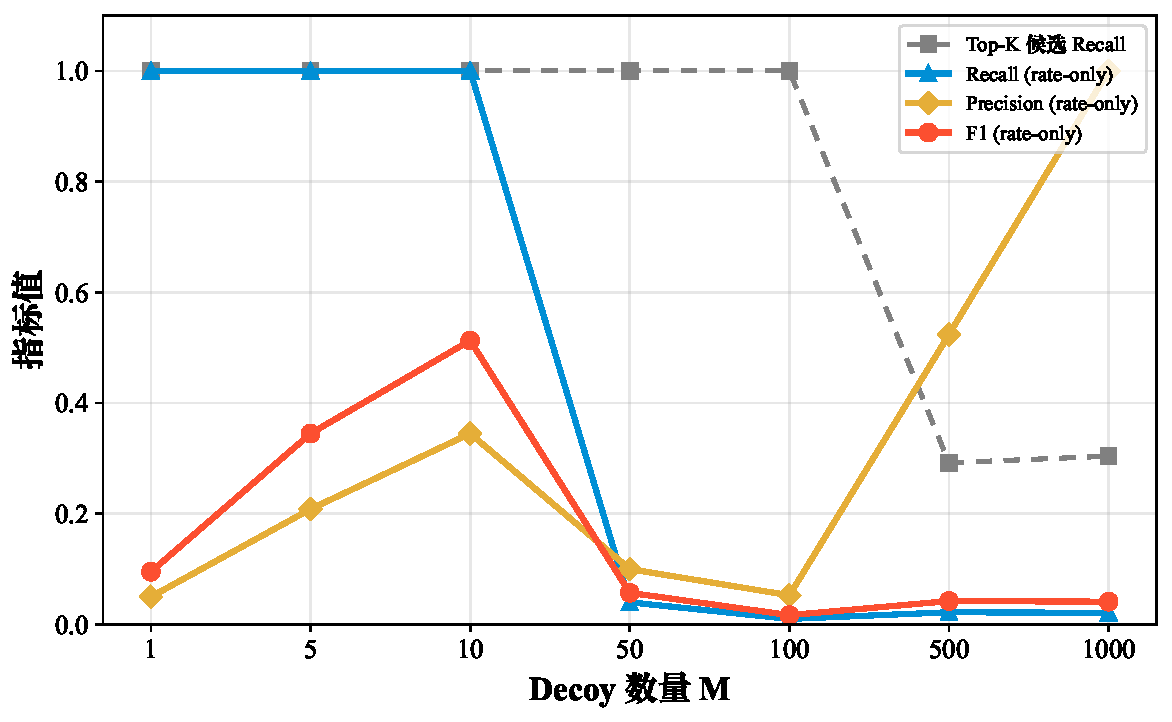
\includegraphics[width=0.48\linewidth]{figs/ch3/fig3_2a_topk_f1.pdf}%
  }%
  \hfill
  \subfloat[S0(rate-only) vs S1(+FO/FI) 的 F1 对比]{%
    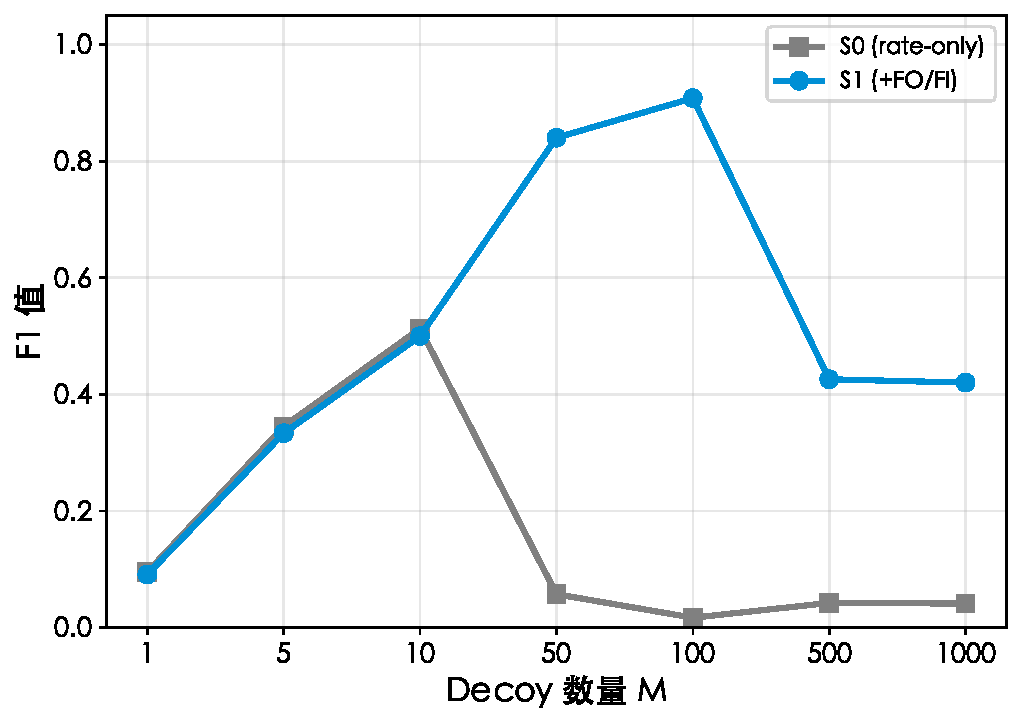
\includegraphics[width=0.48\linewidth]{figs/ch3/fig3_2b_degrade_f1.pdf}%
  }
  \caption{退化攻击下的检测性能。(a) 仅靠聚合速率（rate-only）的一级候选 Recall、阈值判决 Recall/Precision/F1 随 decoy 数 $M$ 的变化；(b) rate-only (S0) 与引入 FO/FI 后 (S1) 的 F1 对比，展示 FO/FI 特征在静态退化场景下的作用。ground truth 以 decoy 目的地址为 key。}
  \label{fig:ch3_fig2_f1}
\end{figure}

\subsection{结果分析：退化证据链与多签名收益}

\noindent\textbf{（1）可分性分析与一级候选诊断}\quad
图~\ref{fig:ch3_fig1_cdf} 从分布层面验证了速率可分性随 $M$ 退化的完整过程。$M=1$ 时，良性 $p_{99}\approx485$~Mb/s 与攻击聚合速率 $10{,}024$~Mb/s 之间存在约 $21$ 倍间隙，一级候选生成器可轻松捕获攻击 key。随着 $M$ 增大到 $100$，攻击 key 的 per-key 速率降至 $100$~Mb/s，已完全融入良性长尾区间，速率特征失去区分力。

图~\ref{fig:ch3_fig2_f1}(a) 从检测管线角度进一步诊断了 rate-only 方案的失效模式。该图同时给出一级候选 Recall、阈值判决 Recall、Precision 与 F1 四条曲线。当 $M\leq100$ 时一级候选 Recall 保持 $1.0$，说明候选生成模块在中等退化下仍具备完整的攻击 key 捕获能力；然而阈值判决 Recall 在 $M=50$ 时骤降至 $0.04$，F1 全程不超过 $0.52$，表明 rate-only 方案的瓶颈在于判决阈值无法区分攻击 key 与良性重流 key。当 $M\geq500$ 时，一级候选 Recall 本身亦降至约 $0.3$，意味着大量攻击 key 的聚合速率已低于良性 key 而被候选生成器排除。需要说明的是，$M\geq500$ 时 rate-only 的 Precision 出现回升（$M=1000$ 时达 $1.0$），但这一现象源于 Recall 极低时（$\sim0.02$）判为正的 key 集合 $|\widehat{F}|$ 极小，分母缩减导致 Precision 的数值放大，并不反映检测能力的实质改善。

从图~\ref{fig:ch3_fig2_f1}(a) 还可以看到，rate-only 方案的失效不是一步发生的，而是先出现候选仍在、判决先失效，随后再演变为候选与判决同时失效。前一阶段说明，单一速率特征的困难在于即使候选已被捕获，也难以把它们从良性重流中分离出来；后一阶段则表明，当 per-key 速率继续下降后，任何依赖重 key 假设的方案都会先撞上候选覆盖率上限。区分这两类失效模式，有助于解释本文为何把改进重点放在第二级多签名判别上，而非一味扩展一级候选规模。

\noindent\textbf{（2）FO/FI 在静态退化场景下的作用}\quad
图~\ref{fig:ch3_fig2_f1}(b) 对比了 S0（rate-only, $\alpha=1$）与 S1（+FO/FI, $\alpha=\beta=0.5$）的 F1 随 $M$ 的变化，展示了 FO/FI 特征在静态退化场景下的作用。S1 的 F1 曲线大致呈现三段变化：

\begin{itemize}
  \item \textbf{重叠段}（$M\leq10$）：S0$\approx$S1，两条线几乎重合。此时攻击 key 聚合速率$\geq1$~Gb/s，rate-only 已能检出全部攻击 key，FO/FI 不提供额外增益。
  \item \textbf{分离段}（$M=50\sim100$）：S1 大幅超越 S0。$M=50$ 时 S0 F1 骤降至 $0.057$，而 S1 跃升至 $0.84$；$M=100$ 时 S1 达峰值 $0.908$，S0 仅 $0.017$。其机理在于：虽然攻击 per-key 速率（$100\sim200$~Mb/s）已接近良性 $p_{99}$，但每个 decoy 的 fan-in（$\text{FI}=B/M=20\sim40$）仍远高于良性 key 的典型 FI（$1\sim5$），FO/FI 特征提供了有效的判别能力。
  \item \textbf{衰减段}（$M\geq500$）：S1 F1 下降至 $0.42$。攻击 per-key 速率降至 $20\sim35$~Mb/s，部分攻击 key 脱离一级候选集（一级候选 Recall$\sim0.3$），候选集的覆盖率瓶颈成为 S1 F1 的天花板。此外，此时 FI$=|\mathcal{B}|/M=2000/500=4$，已接近良性 key 的典型 FI 上界（$1\sim5$），FI 的区分能力同步退化，进一步限制了 S1 的判别空间。
\end{itemize}

需要指出的是，在所有 $M$ 值下都存在约 $20$ 个良性重流 key（rate=$290\sim606$~Mb/s，FI=$13\sim26$）被误判为可疑。这些 key 对应真实的热门目的地，其 rate 与 FI 都落在良性分布的长尾区域，评分自然会超过阈值 $\tau=0.5$，因此构成了当前参数配置（$\tau=0.5$, $\alpha=\beta=0.5$）下基于 rate+FI 检测器的误报基线。调整 $\tau$ 可以改变该数值，但也会影响 Recall（详见消融实验 \S\ref{sec:ch3_eval_ablation}）。这部分误报造成的影响，不在这里预设为可接受或不可接受，而是通过图~\ref{fig:ch3_fig4_attackstate}(d) 的良性吞吐比例结果加以量化。

图~\ref{fig:ch3_fig2_f1}(b) 表明，FO/FI 的优势主要集中在这样一段区间：速率特征已经开始失真，但攻击相关 key 还没有完全跌出候选集。对本章而言，这一点很重要，因为它说明 MS-SatShield 的收益主要来自候选内结构判别能力的恢复，而不是对极端碎片化攻击的完全免疫。当 $M$ 继续增大，FI 也回落到良性区间时，本方法仍会受到一级覆盖率与结构可分性两方面边界的限制。

\noindent\textbf{（3）持续性特征在动态攻击场景下的价值}\quad
图~\ref{fig:ch3_fig2_f1}(b) 仅展示 S0 与 S1 的对比，未包含 S2（+persist）。其原因在于：在静态退化场景中，攻击 key 在每个 epoch 均进入一级候选集，导致持续性 $\widetilde{P}\approx1.0$；同时约 $20$ 个良性重流 key 也几乎每个 epoch 进入候选集，$\widetilde{P}$ 同样趋近 $1.0$，持续性特征对两者加分相同，无法提供额外区分能力。

持续性的作用主要体现在动态退化场景中。为此，图~\ref{fig:ch3_fig4_attackstate} 给出了脉冲式 on-off 攻击下的时域响应。实验固定退化强度为 $M=100$，前 $5$ 个 epoch 为 warmup，随后攻击按 on/off 各 $10$ 个 epoch 的节律周期性切换，总仿真时长为 $100$ 个 epoch。图中红色阴影表示攻击 on-phase；图~\ref{fig:ch3_fig4_attackstate}(a) 给出目标链路利用率，图~\ref{fig:ch3_fig4_attackstate}(b) 给出一级候选命中的攻击 key 数量，图~\ref{fig:ch3_fig4_attackstate}(c) 和图~\ref{fig:ch3_fig4_attackstate}(d) 分别给出 S0、S1、S2 三种方案的 Recall 与良性吞吐比例时域曲线。

\begin{figure}[!htb]
  \centering
  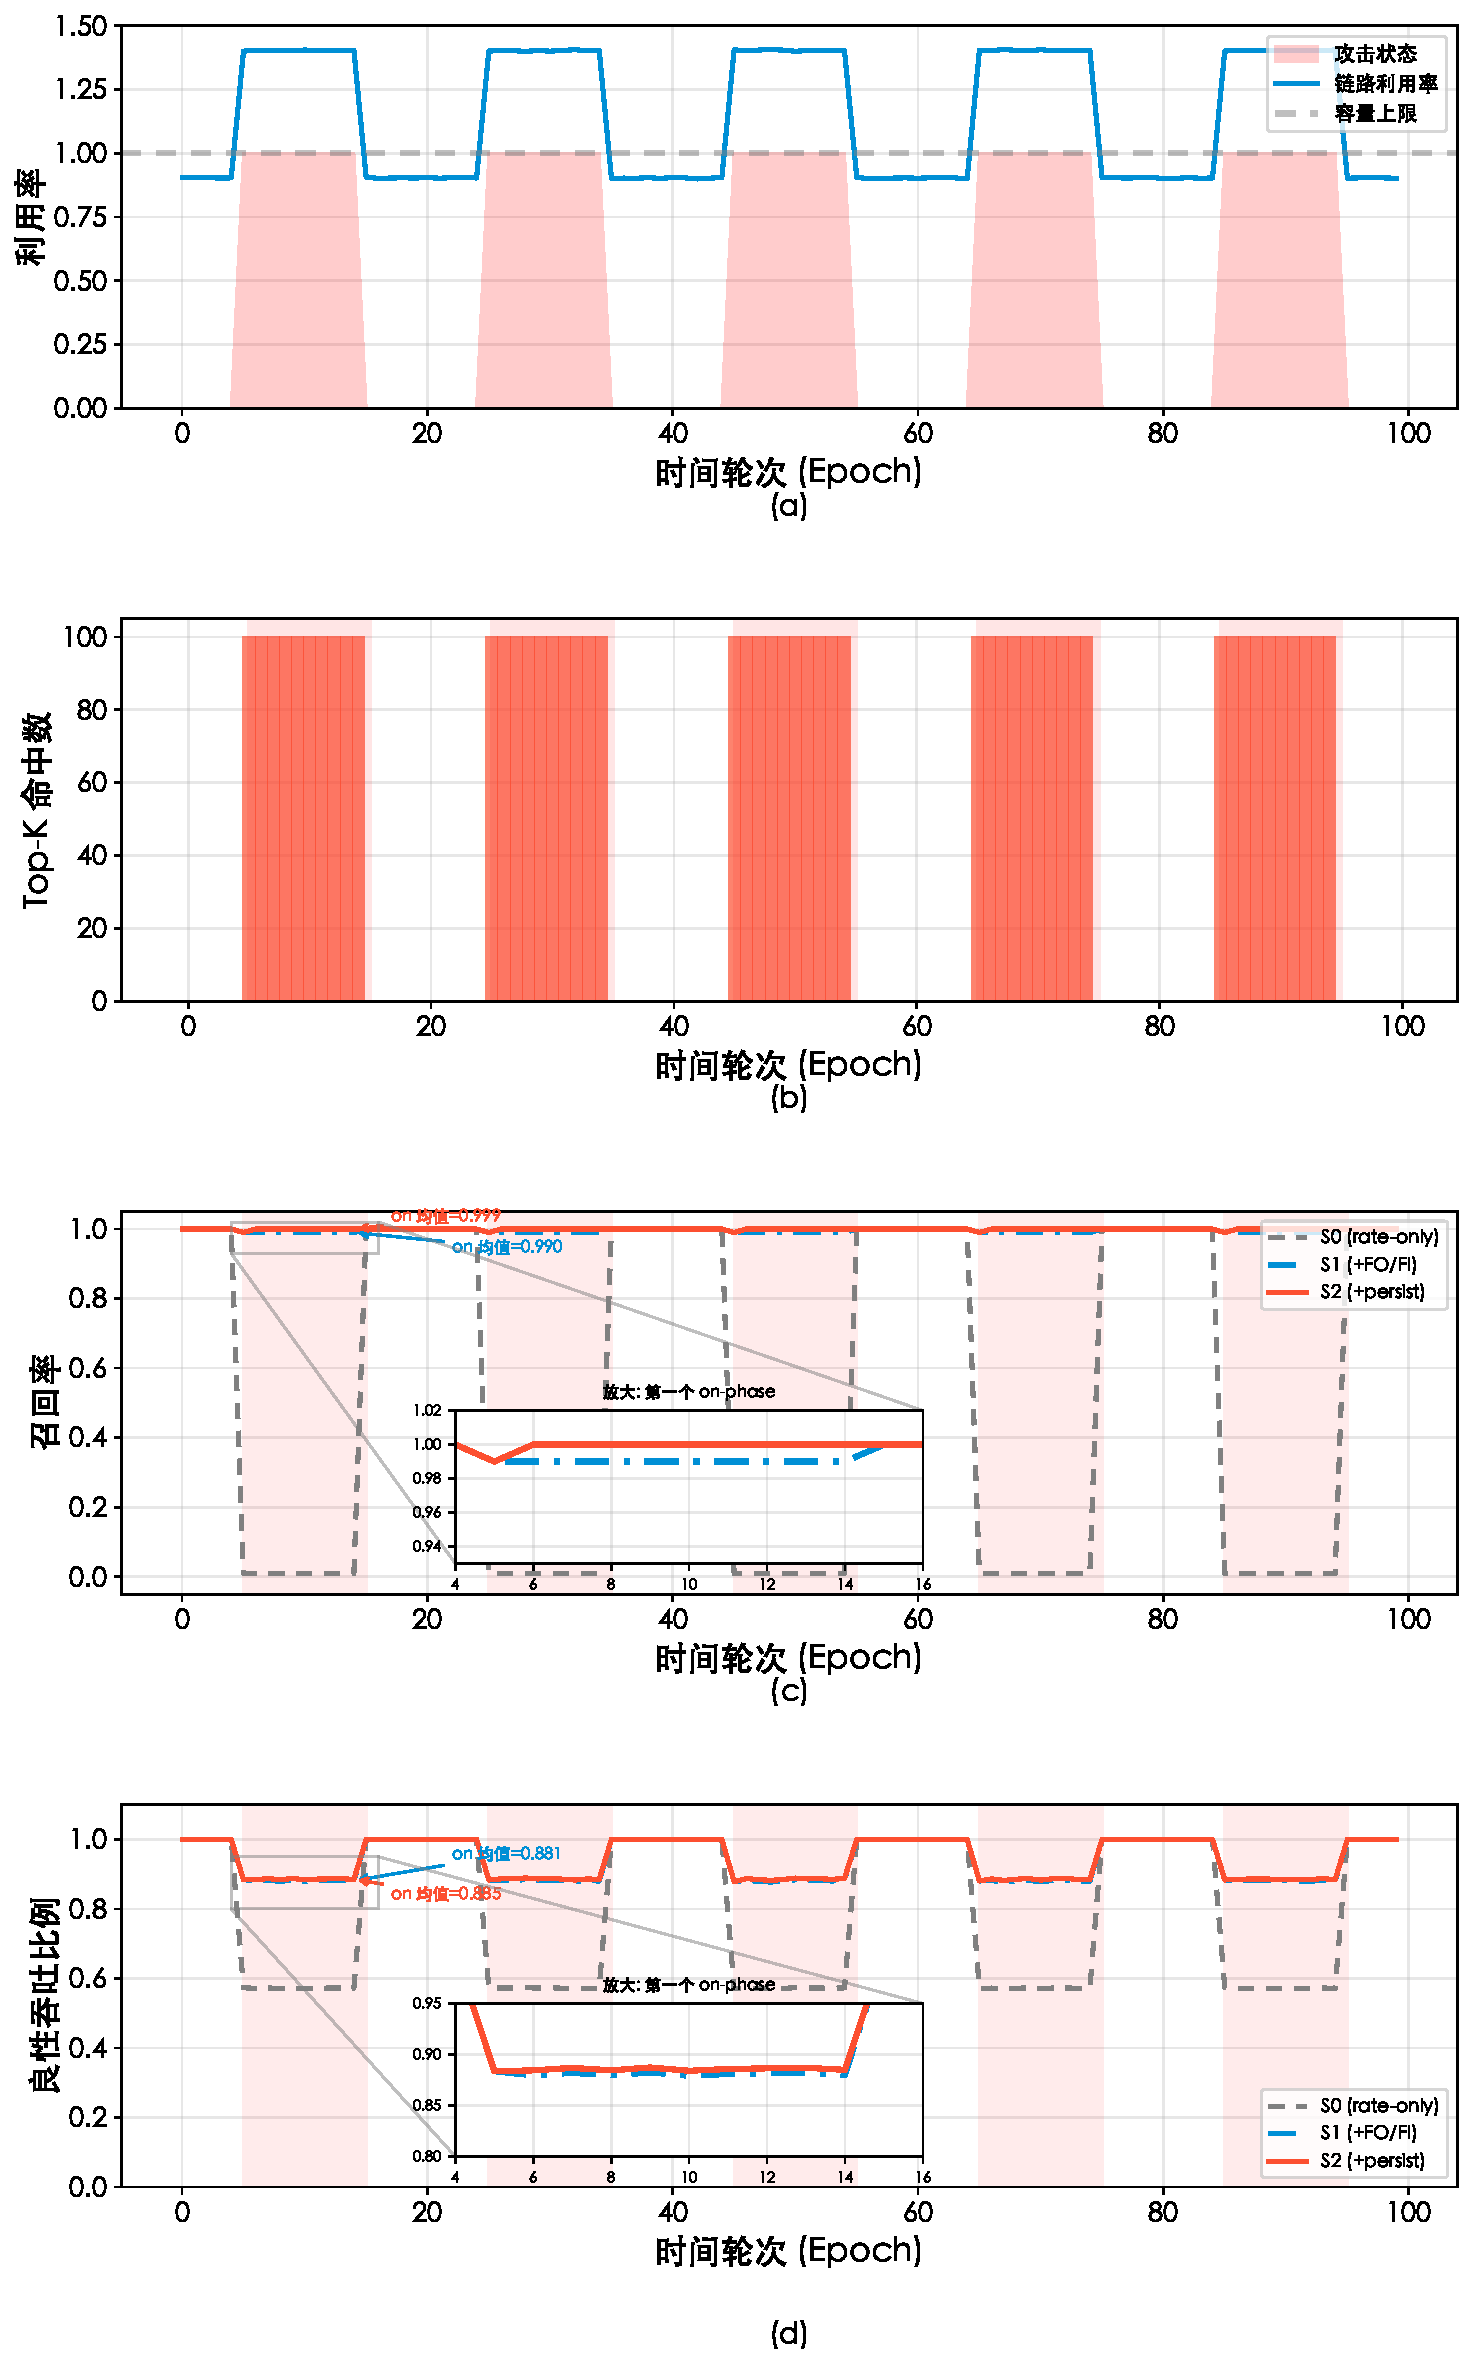
\includegraphics[width=0.94\linewidth]{figs/ch3/fig3_4_onoff.pdf}
  \caption{脉冲式 on-off 攻击下的时域响应对比（$M=100$）。红色阴影表示攻击 on-phase；(a) 目标链路利用率随 epoch 的变化；(b) 一级候选命中的攻击 key 数量；(c) S0、S1、S2 三种方案的 Recall 时域曲线；(d) 三种方案下良性吞吐比例的时域曲线。S2 通过持续性加性奖励与历史候选扩展机制，在候选抖动处保持了更平滑、更高的检测与吞吐保护效果。}
  \label{fig:ch3_fig4_attackstate}
\end{figure}

图~\ref{fig:ch3_fig4_attackstate} 的结果较为清楚。图~\ref{fig:ch3_fig4_attackstate}(a) 表明，攻击 on-phase 到来时目标链路利用率迅速升至超载区间，off-phase 又回落至正常水平，说明该设定确实对应时域上的动态退化，而不是前文的静态退化场景。图~\ref{fig:ch3_fig4_attackstate}(b) 则表明，一级候选集在 on/off 切换附近存在明显抖动：on-phase 内命中数接近攻击 key 总数，但在切换边界处会短暂回落，这正是持续性特征要补偿的部分。进一步看检测结果，图~\ref{fig:ch3_fig4_attackstate}(c) 中 S0 在 $M=100$ 下几乎完全失效（on-phase 平均 Recall$\approx0.01$）；S1 借助 FO/FI 可以实现高召回检测（on-phase 平均 Recall$\approx0.990$），但在切换边缘仍会因候选抖动出现轻微波动；S2 则进一步将 on-phase 平均 Recall 提升到 $0.999$。这里还需说明，off-phase 不存在攻击 key，Recall 按空真值 convention 记为 $1.0$，仅用于保持时域曲线连续。

S2 的提升来自两个机制叠加。持续性采用加性奖励权重（$\alpha=\beta=0.5$, $\gamma=0.2$），即 $\gamma$ 作为额外加分而不从基础权重中借用，因此 S2 的基础检测能力与 S1 保持一致。与此同时，当 $\gamma>0$ 时，系统会将历史上 $P\geq2$ 但未进入当前一级候选集的 key 也纳入评分候选集（见算法~\ref{alg:ms_satshield} 中的持续性扩展步骤），从而为短暂跌出候选集的可疑 key 保留一段记忆。这个机制在缓解侧也有体现：图~\ref{fig:ch3_fig4_attackstate}(d) 显示 S0 的良性吞吐仅为 $0.572$，S1 恢复到 $0.881$，S2 进一步提升到 $0.885$。此外，由于本文取 $k_p=5$，在 off 持续 $10$ 个 epoch 后，所有攻击 key 的 $P_t(a)$ 都会衰减为 $0$，持续性分数随之归零，因此不会把历史攻击残留带入后续判决。

从时域角度看，S2 的改进也主要集中在 on/off 边界，而不是稳态阶段。换句话说，persist 不会把原本不可分的静态样本变得可分，它做的是用跨 epoch 的弱记忆平滑短时抖动，减少候选短暂丢失带来的性能下降。这与图~\ref{fig:ch3_fig2_f1}(b) 中 S2 在静态场景下几乎没有额外收益的结果是一致的：persist 解决的是时间连续性问题，而不是静态结构可分性问题。这样一来，第三章的方法边界也会更清楚，并能更自然地引出第四章的网络级协同。

\subsection{消融实验与参数敏感性分析}
\label{sec:ch3_eval_ablation}
为进一步说明仅对一级候选维护 FO/FI 时的资源与精度权衡，本节对候选规模 $K$、位图长度 $m$、epoch 长度 $\Delta$ 三个参数进行敏感性实验。实验固定退化设定为 $M=100$（速率特征开始失效的分界点），采用 S1（$\alpha=\beta=0.5$）方案进行评估。

\begin{figure}[!htb]
  \centering
  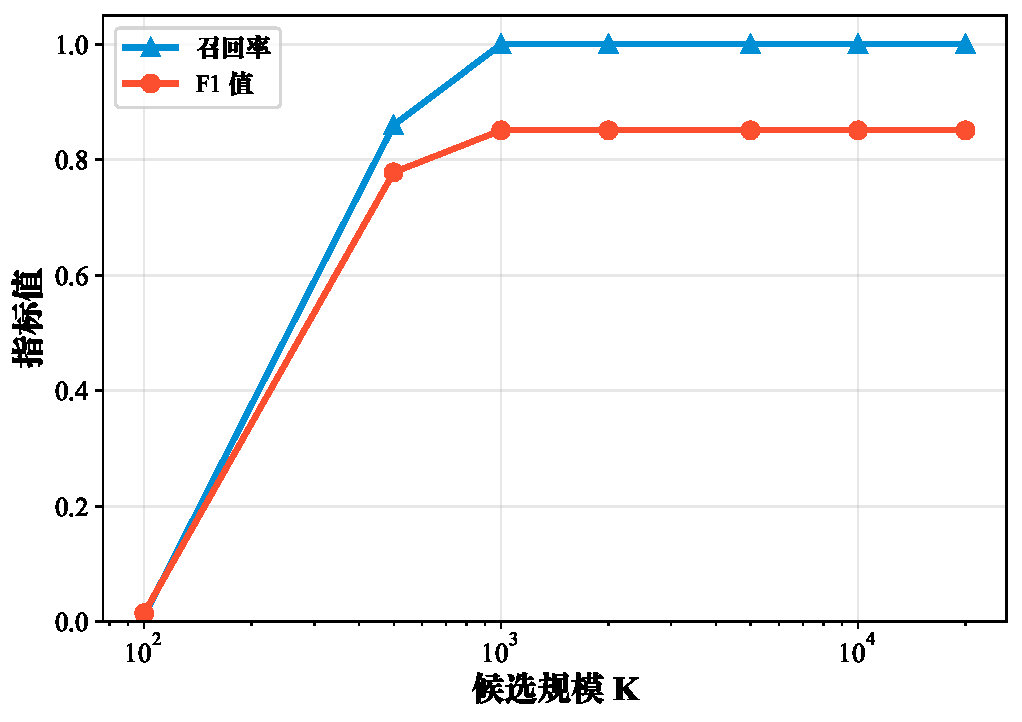
\includegraphics[width=0.65\linewidth]{figs/ch3/ablation_K.pdf}
  \caption{候选规模 $K$ 对 Recall 与 F1 的影响（$M=100$, S1 方案）。$K=1000$ 时 Recall 饱和至 $1.0$，F1 达到约 $0.91$，为推荐的默认值。}
  \label{fig:ch3_ablation_K}
\end{figure}

\noindent\textbf{（1）候选规模 $K$}\quad
图~\ref{fig:ch3_ablation_K} 展示了 Recall 与 F1 随 $K$ 的变化。当 $K<500$ 时，Recall 与 F1 几乎同步上升，这说明此区间内一级候选缓存容量过小，大量攻击 key 尚未进入候选集，是检测性能的主要瓶颈。$K$ 增至 $1000$ 时 Recall 饱和至 $1.0$，F1 达到约 $0.91$。继续增大 $K$（$2000\sim20000$）后 Recall 保持 $1.0$，F1 略有下降（趋近 $0.90$），原因是更多良性 key 涌入候选集增加了误报基数。从资源角度看，若仅计单个 $256$~bit 位图，则 $K=1000$ 时位图本体约为 $K\times m / 8 = 32$~KB；但按本文统一的部署口径，同时计入 CMS 矩阵、候选缓存、FI/FO 双视图、双缓冲位图、字节计数器、rank 表与辅助寄存器后，总状态预算约为 $200$~KB，仍显著低于典型可编程交换机的片上 SRAM 容量。因此 $K\approx1000$（或等效地 $K\approx0.3\cdot N_{\text{keys}}$）是本文实验设置下的经验较优折中。


\noindent\textbf{（2）位图长度 $m$}\quad
图~\ref{fig:ch3_ablation_m} 展示了 FO/FI 估计误差（MAPE）与总内存随 $m$ 的变化。$m=32$ 时 MAPE 约 $4.4\%$，$m=256$ 时降至 $1.1\%$，$m=1024$ 时进一步降至 $0.5\%$。内存开销从 $m=32$ 的约 $20$~KB 线性增长至 $m=1024$ 的约 $700$~KB（$K=1000$ 时）。综合考虑精度与开销，$m=256$ 是本文评估点下经验上较优的折中：MAPE 已降至 $1.1\%$，足以区分攻击 FI（$\geq20$）与良性 FI（$1\sim5$）；按统一部署口径计算，总状态预算约为 $200$~KB，处于可编程交换机可承受范围内。

\begin{figure}[!htb]
  \centering
  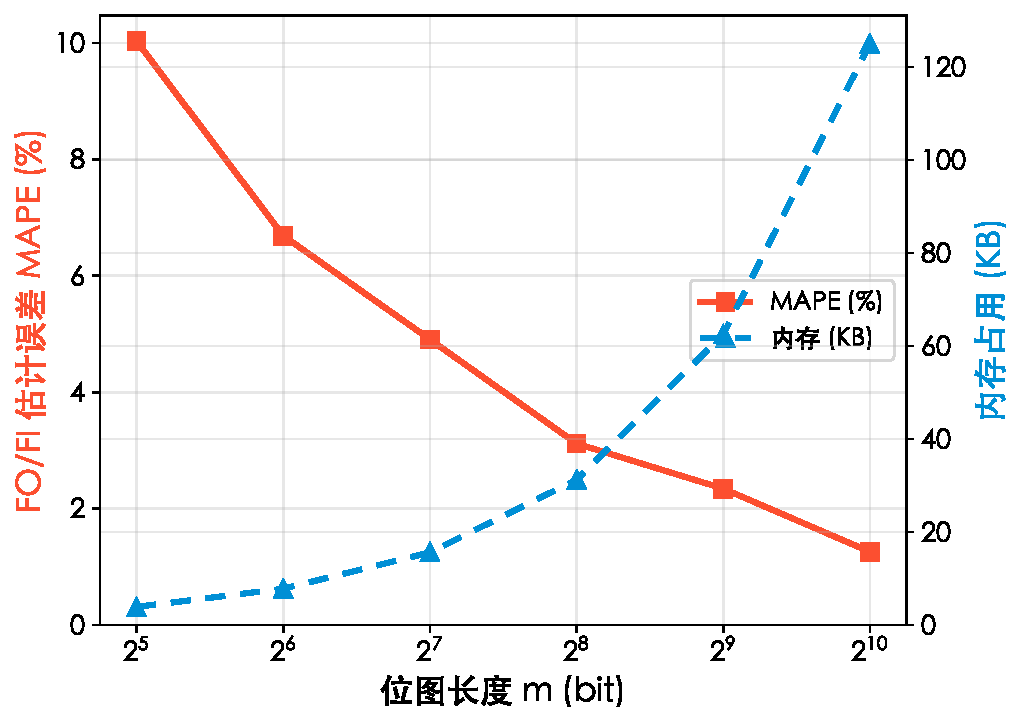
\includegraphics[width=0.65\linewidth]{figs/ch3/ablation_m.pdf}
  \caption{位图长度 $m$ 对 FO/FI 估计误差（MAPE）与总内存的影响（$M=100$, S1 方案）。$m=256$ 时 MAPE 降至 $1.1\%$，内存约 $200$~KB，为推荐的默认值。}
  \label{fig:ch3_ablation_m}
\end{figure}

\noindent\textbf{（3）epoch 长度 $\Delta$}\quad
图~\ref{fig:ch3_ablation_delta} 展示了反应时间与平均良性吞吐下降随 $\Delta$ 的变化。$\Delta=0.1$~s 时反应时间最短（约 $0.2$~s），但代理交互频率高达 $10$ 次/秒，星上计算开销显著增加；$\Delta=5$~s 时反应时间增至 $10$~s，对应良性吞吐下降约 $24\%$。在 $\Delta=0.5\sim1.0$~s 的推荐区间内，反应时间为 $0.5\sim1.0$~s（约 $1\sim2$ 个 epoch），良性吞吐下降约 $12\sim14\%$，系统在响应速度与计算开销之间取得较好平衡。本文选择 $\Delta=1.0$~s 作为默认值。

\begin{figure}[!htb]
  \centering
  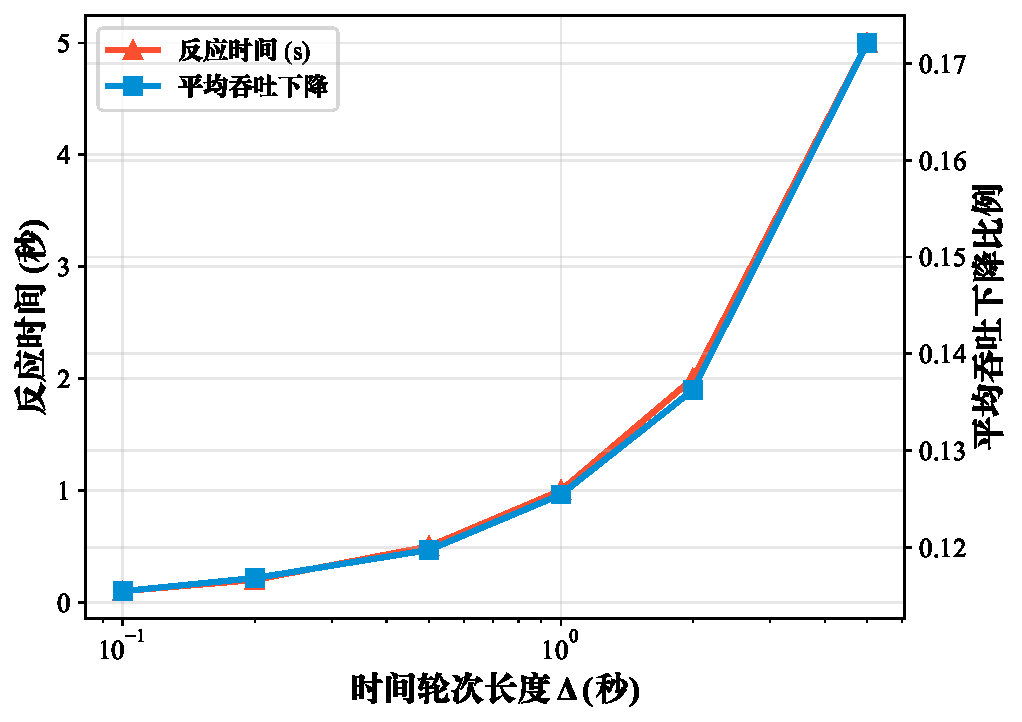
\includegraphics[width=0.65\linewidth]{figs/ch3/ablation_delta.pdf}
  \caption{epoch 长度 $\Delta$ 对反应时间与良性吞吐下降的影响（$M=100$, S1 方案）。$\Delta=1.0$~s 时反应时间约 $1$~s，良性吞吐下降约 $14\%$，为推荐的默认值。}
  \label{fig:ch3_ablation_delta}
\end{figure}

三组消融结果表明，$K$、$m$ 与 $\Delta$ 分别对应三种不同层面的资源约束：$K$ 决定候选覆盖上限，$m$ 决定候选内结构特征的估计精度，$\Delta$ 决定闭环时延与统计稳定性。它们之间并非彼此独立，例如增大 $K$ 会放大位图总开销，缩短 $\Delta$ 会提高 agent 读写频率并加剧候选抖动。因此，本文给出的 $K=1000$、$m=256$、$\Delta=1.0$~s 是面向当前星座规模、链路容量与攻击设定得到的一组经验折中参数。若部署场景发生变化，这三者应被视为联合调参量，而不是彼此孤立的常数。

需要指出的是，地面网络中已经提出了若干针对 LFA 的检测与缓解方案。在 SDN 集中式路线上，Crossfire\citess{crossfire} 利用网络范围内的流量重布局与 SDN 集中控制来检测并解除链路拥塞，Coremelt\citess{coremelt} 利用 NetFlow 分析识别可疑通信对，LinkScope\citess{linkscope} 通过主动探测检测目标链路拥塞，Woodpecker\citess{woodpecker} 和 RADAR\citess{radar} 则分别从路径重路由和相关性分析角度实现 SDN 驱动的 LFA 防御。在可编程数据面路线上，Ripple\citess{ripple} 提出了基于 P4 的去中心化 LFA 防御，Mew\citess{mew} 进一步扩展了 P4 数据面的大规模 LFA 检测能力。然而，这些方案都难以直接应用于 LEO 场景：SDN 集中式方案依赖低时延控制通道与全局视图，而 LEO 的星地和星间控制链路存在明显的时延与带宽限制；P4 方案虽然实现了数据面检测，但依赖地面交换芯片更充裕的片上资源（如 Tofino 2 的 80~MB SRAM），难以满足星载设备的 SWaP 约束。MS-SatShield 的优势在于将检测与缓解逻辑下沉到星载可编程交换机，并在约 $200$~KB 的统一部署状态预算下实现近实时在网缓解。

% [INS-ICARUS-11]
\subsection{方法适用边界与外推限制}
本文方法的第一类边界来自候选覆盖率。实验已经表明，当攻击分散度继续增大（如 $M\geq500$）时，一级候选召回下降会成为主要瓶颈，多签名判别能力也随之受制于候选质量上限。该现象与 ICARUS 在高不确定路由、高分散流量下给出的资源上升但攻击仍可行这一结论并不冲突：二者共同说明，防御侧需要同时改进候选生成与候选内判别，而不能只优化后者\citess{icarus}。

% [INS-ICARUS-12]
第二类边界来自路由策略与网络级目标的差异。本文默认单星本地检测与队列缓解，未显式建模多路径随机负载分担下的概率攻击构造，也未直接评估区域级断连目标。ICARUS 的结果表明，增强路径多样性虽然可以提高攻击成本，但也可能引入显著的时延代价；因此，本文结论应理解为既定路由与本地观测条件下的检测缓解收益，而不应直接外推为全网路由韧性的充分条件\citess{icarus,handley2018delay_not_option,handley2019ground_relays}。

\section{本章小结}
本章针对大规模低轨卫星网络中的链路洪泛攻击，提出了 MS-SatShield 多签名在网检测与队列缓解方法。该方法在 SatShield 的一级候选生成与队列调度框架上，引入 fan-in/fan-out 与持续性等结构性签名，以应对速率特征退化场景；同时通过仅对候选集合维护 FO/FI 的设计，将 distinct 统计的状态成本控制在 $O(K\cdot m)$，并在统一部署口径下将总数据面状态预算控制在约 $200$~KB（默认 $K=1000$, $m=256$，同时计入 CMS 矩阵、候选缓存、FI/FO 双视图、双缓冲位图、字节寄存器与队列映射表等辅助结构）。

实验结果表明：（1）在多 decoy 分摊退化下（$M=100$），仅靠聚合速率的 S0 方案 F1 降至 $0.017$，引入 FO/FI 后的 S1 方案 F1 恢复到 $0.908$；（2）在脉冲式 on-off 攻击下，持续性特征通过加性奖励与候选集扩展机制将 S2 方案的 on-phase 平均 Recall 提升到 $0.999$，良性吞吐恢复到 $0.885$；（3）消融实验表明，在本文评估设置下，$K\approx1000$、$m=256$、$\Delta=1.0$~s 是检测精度与资源开销之间较合适的一组经验折中参数。

不过，上述结果仍局限于单星、单链路视角。当 $M\geq500$ 时，各方案 F1 都下降到 $0.42\sim0.46$，主要受制于单链路一级候选集的覆盖率瓶颈（一级候选 Recall$\sim0.3$）。此外，单节点缓解只是在拥塞形成后于末端丢弃攻击流量，无法阻止攻击流在上游链路上继续消耗带宽。这些局限也自然引出第四章的研究方向：通过多星协同的证据融合与逐跳推回机制，在网络级实现更早、更充分的攻击缓解。



%========================
% 第四章：研究点 2（多星协同在网计算）
% 章节主题：面向大规模低轨卫星网络的抑制型邻居扩散协同与推回缓解
%========================
